\chapter{Sphère isotherme en boîte\label{SIB::Chapitre}} %{Les diagrammes d'énergie et de \textsc{Milne} pour une sphère isotherme en boîte}
%		\markboth{\MakeUppercase{\chaptername}\ \thechapter.\ Diagramme}{}
	\minitoc

	\section{Diagramme de \textsc{Milne}}
		\subsection{Présentation du problème}
	Comme nous l'avons vu dans le chapitre précédent, les sphères isothermes ne sont pas une solution satisfaisante, du fait de leurs masses infinies.
	Nous allons présenter dans ce chapitre une solution de sphère isotherme intégrée sur un support borné. Cette solution est toujours obtenue en recherchant des maxima  de l'entropie statistique de \textsc{Boltzmann} :
	\begin{align*}
		S(f) = - k_B \int f \ln f d\Gamma
	\end{align*}
	mais pour une fonction $f$ possédant un support borné. Ce dernier est par exemple une boule (~souvent appelée boîte, d'où le nom du chapitre~) définie comme :
	\begin{align}
		B = \left\{ \vec{r} \in \mathbb{R}^3\ ;\ \left|\vec{r}\right| < R\right\}
	\end{align}
	où $R$ est le rayon de la boule support de $f$. Dans la suite, nous noterons $\mathbb{I}_{B_R}$ la fonction indicatrice sur cette boule.

\subsection{Obtention des équations}
	La fonction de distribution d'une sphère isotherme en boîte, s'écrit (~voir par exemple \cite{CoursJP}~) :
	\begin{eqnarray}
		f^+(E) = \left(\frac{2\pi\alpha^2m}{\beta}\right)^{-3/2}e^{-\beta E}\times\mathbb{I}_{B_R}
	\end{eqnarray}
	où $\alpha$, en mètre, et $\beta=(k_B T)^{-1}$, en Joule, sont des multiplicateurs de \textsc{Lagrange} imposés par les contraintes respectives de masse $M$ et d'énergie totale $H$ finie que l'on impose au système.
	Ils assurent également la normalisation de la fonction de distribution.
	La quantité \mbox{$E = \frac{p^2}{2m} - m\psi(r)$} est l'énergie d'une particule test de masse $m$ se déplacant dans
	le potentiel $\psi$ créé par la sphère isotherme.
	Le calcul de la densité de masse donne alors \mbox{$\rho(r) = \frac{m}{\alpha^3}e^{-\beta m \psi(r)}\times\mathbb{I}_{B_R}$}. % \psi'(r)}$}, dans la suite nous utiliserons :
	%\mbox{$\psi'(r) = \psi(r) - \psi(0)$}~\footnote{pour faciliter les calculs dans les variables \textsc{Milne} définies ci-dessous}.
	L'équation de \textsc{Poisson} s'écrit :
	\begin{equation}
		 \frac{1}{x^2}\frac{d}{dx}\left(x^2\frac{d h}{dx}\right) = e^{-h} \times\mathbb{I}_{B_R} \notag
	\end{equation}
	où nous avons utilisé l'adimensionnement  :
	\begin{eqnarray}
		x &= \frac{r}{r_0}\mathrm{ avec }\ r_0 = \sqrt{\frac{\alpha^3}{4\pi G m^2\beta}}e^{-\frac{m\beta\psi(0)}{2}} \label{toto11} \\
		h &= m\beta\psi(x) - m\beta\psi(0) \label{toto12}
		\end{eqnarray}
		Il est important de noter que l'inconnue du problème $h(x)$ est différente de $y(x)$ utilisée pour la présentation du problème de la sphère isotherme illimitée. Nous avons ici $h(0) = 0$ alors que $y(0) = m\beta\psi(0)$.
		
		En notant par un $^\prime$ toutes les dérivées par rapport à la variable $x$, on introduit les variables dites de \textsc{Milne :}
		$$\begin{cases}
			v = x \dfrac{d h}{dx} = x \x{h} \\
			\\
			u = \dfrac{e^{-h} x}{h'} = \dfrac{e^{-h} x^2}{v}
		\end{cases}$$ \label{syst_uv}
		
Un calcul simple donne alors :
\begin{equation}
	\dfrac{d(xv)}{dx} = uv \;\;\Rightarrow\;\; \x{v} = \frac{v \left( u - 1\right)}{x} \notag
\end{equation}
La dérivée de $u$ s'obtient directement à partir de sa définition, on trouve :
	$$\begin{cases}
		\x{v} = \dfrac{v \left( u - 1\right)}{x} \\
		\x{u} = \dfrac{u}{x}\left(3 - v - u\right)
	\end{cases} \label{systdudv}$$
	
	que l'on peut écrire de façon compacte
	\begin{equation}
		\fbox{$
		\dfrac{d v}{d u} = \dfrac{v \left( u - 1\right)}{u \left(3 - u - v\right)}
		$} \label{eqdudv}
	\end{equation}
	La courbe résultant de cette équation, tracée dans le plan $\left(u, v\right)$, forme le diagramme
	de \textsc{Milne}. L'étude de ce diagramme permet d'accéder à de nombreuses caractéristiques de la sphère isotherme en boîte. L'équation \ref{eqdudv} ne peut être résolue explicitement mais sa solution peut être obtenue numériquement; il faut pour cela préciser les conditions au bord et au centre du système; c'est l'objet de la section suivante.
	

\subsection{Conditions au centre et sur le bords de la sphère}
	Pour obtenir les conditions initiales permettant la résolution de l'équation~\ref{eqdudv}, nous devons obtenir les conditions aux limites pour la sphère isotherme en boîte.
\subsubsection{En $x = 0$}
	Pour ce faire, nous nous plaçons dans le voisinage de $x=0$, et faisons donc des développements limités de la variable $h$ représentant le potentiel.
	Cela nous permettra d'obtenir le comportement approché de $u(x)$ et de $v(x)$ au centre.
	Nous avons donc :
	\begin{eqnarray*}
		h(x) = h(0) + \x{h}(0)x + \frac{d^2 h}{dx^2}(0)\frac{x^2}{2!} + \frac{d^3 h}{dx^3}(0)\frac{x^3}{3!} + o(x^3) = ax^2 + bx^3 + o(x^3)
	\end{eqnarray*}
	En effet, \mbox{$h(0) = m\beta\left(\psi(0) - \psi(0)\right) = 0$} et \mbox{$\x{h}(0) = m\beta\x{\psi}(0) = 0$} car \mbox{$\x{\psi} = r_0\frac{d \psi}{dr}\propto F$},
	$F$ étant la force s'appliquant sur la particule test.
	Au centre de la sphère, les forces qui s'appliquent à une particule test s'opposent les unes aux autres, d'où $\x{h}(0) = 0$.

	Les variables $u$ et $v$ vont alors se développer comme :
	\begin{eqnarray}
		v &=& x\x{h} = 2ax^2 + 3bx^3 + o(x^3)\label{vDL} \\
		u &=& \frac{x^2e^{-ax^2 - bx^3 + o(x^3)}}{2ax^2 + 3bx^3 + o(x^3)} \\
		  &=& \frac{1 - ax^2 - bx^3 + o(x^3)}{2a + 3bx +o(x)} \\
		  &=& \frac{1}{2a} - \frac{3b}{4a^2}x + o(x)\label{uDL}
	\end{eqnarray}
	Nous utilisons ensuite l'équation de Poisson pour déterminer, par identification, les valeurs de $a$ et de $b$ :
	\begin{eqnarray}
		\x{\left(xv\right)} = 6ax^2 + 12bx^3 + o(x^3) = uv = x^2 + o(x^3)\label{PoisDL}
	\end{eqnarray}
	D'où :
	\begin{eqnarray}
		\left\{\begin{array}{l}
			a = \frac{1}{6} \\
			b = 0
		\end{array}\right.
	\end{eqnarray}
	Maintenant que nous avons nos développements, nous en déduisons les conditions initiales :
	$$(u,v) \substack{\longrightarrow \\ r\to 0} (3,0)$$

\subsubsection{Sur le bords de la sphère : $r = R$}
	Soit $X = \frac{R}{r_0}$. Nous allons tenter d'exprimer nos variables $u$ et $v$ au point $X$ en fonction des quantités connues du problème,
	telles que l'énergie totale $H$, la masse totale $M$, le rayon de la sphère $R$.
	Et, selon la description canonique ou micro canonique choisie, en fonction de la température cinétique du système.

	On introduit les constantes adimensionnées suivantes :
	\begin{eqnarray*}
		\left\{\begin{array}{l}
			\lambda = - \frac{H R}{G M^2} \\
			\\
			\mu     = \frac{m\beta GM}{R}
		\end{array}\right.
	\end{eqnarray*}
	où $\lambda$ représente l'énergie adimensionnée et $\mu$ l'inverse de la température adimensionnée.

	Au bord du système, nous pouvons écrire que $\frac{d \psi}{dr} \equiv \frac{GM}{R^2}$~\footnote{Théorème de Gauss}. De plus :
	\begin{eqnarray*}
		\x{h}(X) = m\beta r_0 \frac{d \psi}{dr} = m\beta r_0 \frac{GM}{R^2} = \frac{\mu}{X} \Rightarrow \mu = X\x{h}(X)
	\end{eqnarray*}
	Or $v(X) = X\x{h}(X)$, d'où :
	\begin{eqnarray}
		v\left(X\right) := v_m = \mu\label{vmmu}
	\end{eqnarray}

	Il nous reste l'énergie à exprimer.
	Pour cela, nous allons commencer par calculer l'énergie totale $H$ à l'aide du théorème du Viriel adapté à une sphère isotherme en boîte~\footnote{Pour un système tronqué, le calcul permettant d'arriver au théorème du Viriel fait apparaître des termes dû aux intégrations par partie qui vont rester.} :
	\begin{eqnarray}
		2T + W = \frac{4}{3}\pi R^3 P_e
	\end{eqnarray}
	avec $P_e$ la pression qui s'exerce sur le bord de la sphère.
	L'énergie cinétique s'écrit \mbox{$K = \frac{1}{2}mv^2 = \frac{3}{2} N k_B T = \frac{3}{2} \frac{M}{m} k_B T$}.
	Donc :
	\begin{eqnarray*}
		H &=& K + W = \frac{3}{2} \frac{M}{m\beta} + \frac{4}{3}\pi R^3 P_e - 2K \\
		  &=& -\frac{3}{2} \frac{M}{m\beta} + \frac{4}{3}\pi R^3 P_e \\
		\Rightarrow \lambda &=& \frac{3}{2}\frac{MR}{m\beta GM^2} - \frac{4}{3}\pi R^3 P_e \frac{R}{GM^2}
	\end{eqnarray*}
	Une sphère isotherme est un système barotropique. Elle a donc une équation d'état polytropique d'indice 1 : $P = \frac{\rho(r)}{m\beta} \Rightarrow P_e = \frac{\rho(R)}{m\beta}$ que nous remplaçons :
	\begin{eqnarray}
		\lambda &=& \frac{3}{2}\frac{1}{X\x{h}(R)} - \frac{4}{3}\pi R^3 \frac{\rho(R)}{m\beta} \frac{R}{GM^2} \notag \\
			&=& \frac{3}{2}\frac{1}{X\x{h}(R)} - \frac{4}{3}\pi R^3 \frac{e^{-h(R) + m\beta\psi(0)}}{\alpha^3\beta} \frac{R}{GM^2} \notag \\
			&=& \frac{3}{2}\frac{1}{X\x{h}(R)} - \frac{4}{3}\pi R^3 \frac{4\pi G \beta m^2 e^{\beta m \psi(0)}}{\alpha^3} r_0^2\frac{e^{-h(R)}}{(\x{h}(R))^2} \notag \\
			&=& \frac{3}{2}\frac{1}{X\x{h}(R)} - \frac{e^{-h(R)}}{(\x{h}(R))^2}\label{lamum}
	\end{eqnarray}

	Nous avons ensuite, par substitution, les valeurs maximales $u_m$ et $v_m$ de $u$ et $v$ en fonction des paramètres du problème :
	\begin{eqnarray}
		\label{uv_max}
		\fbox{$
		\left\{\begin{array}{l}
			v_m = \mu \\
			u_m = \frac{3}{2} - \lambda \mu
		\end{array}\right.
		$}
	\end{eqnarray}



\subsection{Droites de \textsc{Padmanabhan} et diagramme de \textsc{Milne}}
	On peut facilement éliminer $\mu$ dans le système \ref{uv_max} et obtenir
	\begin{equation}
		v_m = \frac{3}{2\lambda} - \frac{u_m}{\lambda}\label{droitePb}
	\end{equation}
	Cette relation montre que si l'on ne fixe que la valeur de $\lambda$,  les couples $(u_m,v_m)$  se répartissent dans le plan $(u,v)$ le long d'une droite de pente $-1/\lambda$, dite de \textsc{Padmanabhan} en référence à sa remarque dans l'article \cite{1989ApJS...71..651P}. On remarque aussi que toutes ces droites passent par le point $(\frac{3}{2},0)$.
	
	Le choix de $\lambda$ est indépendant de la valeur de la température, le point $(u_m,v_m)$ associé à la sphère isotherme en boite de rayon $R$, de masse $M$, d'énergie $H$ et de température $\beta$ se trouve donc à l'intersection de la droite de Padmanabhan fixée par $\lambda$ et de la courbe v(u) solution de l'équation \ref{eqdudv}. 
	
	
	Cette courbe est obtenue numériquement à l'aide d'un solveur RK4, en utilisant les variables adimensionnées le seul paramètre physique pour la résolution est la valeur de $X$ caractérisant le rayon et la température de la sphère.  L'ensemble de ces courbes et des droites de Padmanabhan correspondantes sont représentées sur la figure \ref{Milne}. Pour une température fixée, on constate que plus la valeur de $R$ augmente plus la courbe solution est longue et finit par s'enrouler dans une spirale convergeant vers un point. Ce point correspond au cas $R\to\infty$ et donc celui de la SIS.
	
	\'{A} la l'inspection de ce diagramme et de ces droites, on comprend aisément que l'on ne peut pas mettre n'importe quelle sphère isotherme dans n'importe qu'elle boîte !
	En effet, si l'on impose des valeurs de $R$, $M$ et $H$ qui donnent une valeur trop grande $\lambda>\lambda_c$, la droite ne pourra pas avoir d'intersection avec la courbe. Cette intersection qui aurait fixé le dernier paramètre, la température, n'existant pas il en va de même de la sphère isotherme en boîte possédant ces caractéristiques physiques.
	
	On remarque même l'existence d'une seconde valeur caractéristique $\lambda_0$ telle que :
	\begin{itemize}
		\item si $\lambda < \lambda_0$ : il n'existe qu'une seule et unique sphère isotherme possible;
		\item si $\lambda \in \left[\lambda_0,\lambda_c\right]$ : il existe plusieurs possibilités;
		\item si $\lambda > \lambda_c$ : il n'y a plus d'intersection possible !
	\end{itemize}

Comme nous allons le voir dans la prochaine section, cette multiplicité de possibilité est associée à la stabilité des sphères concernées.

	\begin{figure}[h!]
		\begin{minipage}[b]{0.40\linewidth}
			\centering \includegraphics[scale=0.60]{graphe/r_max-1.pdf}
		\end{minipage}\hfill
		\begin{minipage}[b]{0.48\linewidth}
			\centering \includegraphics[scale=0.60]{graphe/r_max-5.pdf}
		\end{minipage}
		\begin{minipage}[b]{0.40\linewidth}
			\centering \includegraphics[scale=0.60]{graphe/r_max-10.pdf}
		\end{minipage}\hfill
		\begin{minipage}[b]{0.48\linewidth}
			\centering \includegraphics[scale=0.60]{graphe/r_max-300.pdf}
		\end{minipage}
		\caption{Diagramme de \textsc{Milne} pour $X=1$, $X=5$, $X=10$ et pour $X=300$}
		\label{Milne}
	\end{figure}

	\section{Diagramme d'énergie}
		\subsection{Diagramme}
	Le diagramme n°~\ref{Ener} a été tracé à l'aide de la même résolution numérique que le diagramme de \textsc{Milne}.
	En effet, à la sortie de la résolution, nous connaissions les coordonnées du point $\left(u_m,v_m\right)$.
	Connaissant ces valeurs et leurs expressions théoriques en fonction des paramètres du système,
	nous pouvons remonter aux variables adimensionnées $\lambda$ et $\mu$ à l'aide des relations \ref{vmmu} et \ref{lamum}.
	Ces variables représentant physiquement l'inverse de la température cinétique du système (~$\mu$~) et l'énergie totale du système (~$-\lambda$~),
	nous les utilisons pour remonter à ce diagramme, constituant un diagramme de stabilité.
	\textcolor{red}{\underline{Attention :}} sur ce graphe est tracée la courbe $\mu\left(-\lambda\varpropto H\right)$.
	\begin{figure}[h!]
		\centering \includegraphics[scale=1.00]{graphe/energie.pdf}
		\caption{Diagramme d'énergie/stabilité}
		\label{Ener}
	\end{figure}

	Dans le diagramme de \textsc{Milne}, la sphère isotherme singulière correspondait au point $\left(1,2\right)$.
	Dans ce diagramme, elle va correspondre au point $\left(\lambda = \frac{u_m - 3/2}{v_m} = -1/4, \mu = v_m = 2\right)$.
	De la même manière que sur le diagramme précédent, la courbe tend en spiralant vers la sphère isotherme singulière, mais avant de l'atteindre,
	elle passe par un minimum de température, puis un maximum d'énergie. Ces deux diagrammes sont équivalents et complémentaires.

\subsection{Stabilité de la sphère isotherme en boîte}
	En physique statistique, il existe deux ensembles capables de décrire la sphère isotherme telle que nous l'avons construite :
	\begin{enumerate}
		\item l'ensemble micro canonique : nous fixons l'énergie totale de la sphère, et nous en déduisons la température cinétique.
		\item l'ensemble canonique : cette fois, l'énergie est laissée libre mais la
			température est fixée.
			A l'équilibre, nous déduisons l'énergie de la température.
	\end{enumerate}

	Le diagramme d'énergie (~figure~\ref{Ener}~) montre deux tangentes (~une verticale et une horizontale~) :
	au-delà de ces tangentes, des questions sur la stabilité commence à se poser : nous avons tronqué la SIS en la mettant dans une boîte ; ce faisant, nous avons introduit
	des contraintes sur les valeurs d'énergie et de température possible, contraintes représentées par les tangentes horizontale et verticale.
%	Si la sphère à une température tel que l'on soit au-dessus de la tangente horizontale, il n'y a plus
%	de sphère isotherme en boîte possible.
	Nous comprenons alors qu'il n'est pas possible de choisir arbitrairement la température d'une sphère isotherme en boîte et qu'il existe une température minimale pour ce type de système.
	\textsc{Katz} a montré qu'il s'agissait en fait d'une limite d'énergie (~voir~\cite{Katz-Stab}~).
	La tangente horizontale nous donne la température minimale permettant de construire une sphère isotherme en boîte
	stable. Le raisonnement est identique pour la tangente verticale conduisant à une énergie minimale.
	Ces tangentes sont tracées sur la figure~\ref{Ener-tg}.
	\begin{figure}[h!]
		\centering \includegraphics[scale=1.00]{graphe/Energie_tg.pdf}
		\caption{Les tangentes : limites de stabilité}
		\label{Ener-tg}
	\end{figure}

	Nous avons maintenant les énergies et températures limites pour la sphère isotherme en boîte.
	Pour comprendre un peu mieux ce qui se passe, voyons si nous pouvons obtenir la densité de la sphère pour ces valeurs limites.

\subsection{Contraste de densité\label{contraste-dens-SIB}}
	Nous rappelons que la densité de la sphère isotherme s'écrit :
	\begin{equation*}
		\rho(r) = \frac{m}{\alpha^3}e^{-\beta m\psi(r)}
	\end{equation*}
	Commençons par adimensionner la densité.
	Nous allons réutiliser le changement de variable sur le potentiel fait plus haut :
	$h(r) = m\beta\(\psi(r) - \psi(0)\)$,
	puis nous allons poser $\rho^s(r) = \frac{\rho(r)}{\rho_0}$, où $\rho_0 = \frac{m}{\alpha^3}e^{-m\beta\psi(0)}$ est la densité au cœur de la sphère.
	Nous obtenons alors l'équation :
	\begin{equation*}
		\rho^s(r) = e^{-h(r)}
	\end{equation*}
	qui se réécrit facilement dans les variables de \textsc{Milne} :
	\begin{equation}
		\rho^s(x) = \frac{u(x) v(x)}{x^2}
	\end{equation}

	Examinons le comportement de la densité au centre de la sphère et sur son bord externe :
	\begin{itemize}
		\item en $x=0$ : nous réutilisons les développements limités de $u$, $v$ et $uv$ fait plus haut (~équations~\ref{uDL}, \ref{vDL} et \ref{PoisDL}~) :
			\begin{align}
				\rho^s(0) &= \left(x^2 + o\left(x^3\right)\right)x^{-2} \notag \\
					  &= 1 + o\left(x\right) \notag
			\end{align}
		\item en $x=X$ : le résultat arrive assez naturellement :
			\begin{align}
				\rho^s(X) &= u_mv_mX^{-2} \notag \\
					  &= \mu X^{-2}\left(\frac{3}{2} - \lambda\mu\right) \notag
			\end{align}
	\end{itemize}

	Nous en déduisons ainsi l'expression du contraste de densité en fonction des paramètres de la sphère :
	\begin{align}
		\R = \frac{\rho(0)}{\rho(R)} &= \frac{\rho^s(0)}{\rho^s(X)} \\
			   &= \frac{X^2}{\mu\left(\frac{3}{2} - \lambda\mu\right)}
	\end{align}

	Lors de la résolution numérique du système, il a été obtenu que les valeurs de $\mu$ et $\lambda$ pour ces limites sont :
	\begin{itemize}
		\item Pour la tangente verticale : $\(\lambda, \mu\) = \left(-0.33457, 2.03152\right)$ pour $X = 34.2999$.
			%$\left(\mu, \lambda\right) = \left( 2.034753, -0.334562 \right)$ et $X = 33.99$.
			D'où un contraste de densité de $\R^H_c \thickapprox 705.967$.
		\item Pour la tangente horizontale : $\(\lambda, \mu\) = \left(-0.19876, 2.51755\right)$ pour $X = 8.9999$.
			%$\left(\mu, \lambda\right) = \left( 2.51755, -0.19874 \right)$ et $X = 8.99$.
			D'où un contraste de densité de $\R^\beta_c \thickapprox 32.186$.%16.081$.
	\end{itemize}
	L'instabilité intervient quand le système dépasse l'une de ces valeurs de contraste, selon que nous ayons imposé la température ou l'énergie.
	Ainsi, les descriptions canonique et microcanonique ne sont pas équivalentes.

%	Nous avons maintenant réduit l'étude d'une sphère isotherme en boîte à une seule quantité : le contraste de densité.
	Nous avons maintenant exprimé les limites de stabilité s'appliquant à la sphère isotherme en boîte en terme d'énergie, de température, et de contraste de densité.
	Après tous ces développements, nous résumons les paramètres utiles d'une sphère isotherme et le passage des quantités utilisées ici
	à des quantités plus physiques dans les tableaux~\ref{SIB:important} et~\ref{SIB:lien}.
	\begin{table}[h]
		\begin{center}
			\begin{tabular}{|c|c|}
				\hline
				Paramètres	&	Description \\
				\hline
				\hline
				$\R_c$		&	\textbf{Contraste de densité :} dépend du rayon de la sphère isotherme. \\
						&	Il nous donne des informations sur la stabilité de l'objet. \\
				\hline
				$X = R/r_0$	&	\textbf{Rayon de la sphère :} paramètre dont dépend toutes les informations physiques \\
						&	sur l'objet (~position dans les différents diagrammes, contraste de densité~). \\
				\hline
			\end{tabular}
			\caption{Paramètres importants\label{SIB:important}}
		\end{center}
	\end{table}

	\begin{table}[h]
		\begin{center}
			\begin{tabular}{|c|c|}
				\hline
				Quantité physique	&	Lien avec le modèle \\
				\hline
				\hline
				Distance au centre $r$	&	$r = r_0 x$ \\
				\hline
					&	\\
				Densité $\rho(r)$	&	$\rho(r) = \dfrac{m}{\alpha^3}\dfrac{u v}{x^2}$ \\
					&	\\
				\hline
				Potentiel $\psi(r)$	&	\mbox{$\psi(r) = h + m\beta\psi(0)$} \\
							&	\mbox{$ h = -\ln\(\dfrac{u v}{x^2}\) $} \\
							&	\mbox{$ \Rightarrow \psi(r) = -\ln\(\dfrac{u v}{x^2}\) + m\beta\psi(0)$} \\
				\hline
			\end{tabular}
			\caption{Lien entre les paramètres physiques et les variables de \textsc{Milne}\label{SIB:lien}}
		\end{center}
	\end{table}


	L'état d'une sphère isotherme en boîte (~diagramme de \textsc{Milne}, densité, position sur le diagramme d'énergie et contraste de densité~)
	est tracée sur la figure~\ref{Sphere}.
	La courbe de densité fait clairement apparaître un cœur (~$\rho(r) \simeq \mathrm{cte}$~) et un halo (~$\rho(r) \varpropto r^{-\alpha}$~) dont la pente est $\alpha \simeq 2$, qui est celle d'une SIS.
	\begin{figure}[ht!]
		\begin{minipage}[b]{0.40\linewidth}
			\centering \includegraphics[scale=0.60]{graphe/Milne_etat.pdf}
		\end{minipage}\hfill
		\begin{minipage}[b]{0.48\linewidth}
			\centering \includegraphics[scale=0.60]{graphe/Densite_etat.pdf}
		\end{minipage}
		\begin{minipage}[b]{0.40\linewidth}
			\centering \includegraphics[scale=0.60]{graphe/Energie_etat.pdf}
		\end{minipage}\hfill
		\begin{minipage}[b]{0.48\linewidth}
			\centering \includegraphics[scale=0.60]{graphe/Contraste_etat.pdf}
		\end{minipage}
		\caption{État de la sphère isotherme pour $X = 30$}
		\label{Sphere}
	\end{figure}

	Nous allons maintenant étudier la solution proposé par \textsc{King}.


%		\section{Numérique}
%			Écrire partie numérique sur milne, ...


\chapter{Le modèle de \textsc{King}\label{King::Chapitre}}
	\minitoc

	\section{Équation de \textsc{Poisson}}
		%\subsection{Calcul v2.0}

La fonction de distribution associée à ce modèle de King s'écrit (~voir~\cite{King-1966AJ}~) :
\begin{equation}
	f_K(E) = \begin{cases}
		\rho_0 \(2\pi m\sigma^2\)^{-3/2}\( e^{\frac{E_l-E}{\sigma^2}} - 1\) & \text{si $E < E_l$} \\
		0 & \text{si $E > E_l$}
	\end{cases}
\end{equation}
%\begin{equation}
%	f_K(E) = \left\{\begin{array}{l} \rho_0 \(2\pi m\sigma^2\)^{-3/2}\( e^{\frac{E_l-E}{\sigma^2}} - 1\)\ \mathrm{si}\ E < E_l \\
%		\\
%		0\ \mathrm{si}\ E > E_l
%	\end{array}\right.
%\end{equation}
où la dimension de $\sigma^2$ est celle d'une énergie. Ce paramètre représente la dispersion d'énergie du système.
Le paramètre $\rho_0$ est la densité de masse au centre du système. L'énergie $E_l$  de libération d'une particule s'écrit : $E_l = \frac{p_l^2}{2m} + m\psi(r)$, où $\psi(r)$ est le potentiel gravitationnel de la sphère de King et  $p_l$ l'impulsion de libération fonction de $r$.

La densité de masse s'écrit toujours à partir de la fonction de distribution :
\begin{eqnarray*}
	\rho(r) &=& \int^{p_l}_0\,f_K(E)4\pi p^2dp \\
		&=& \frac{\rho_0}{\(2\pi m\sigma^2\)^{3/2}}\int_0^{p_l}\,\left\{e^{\frac{E_l-E}{\sigma^2}} -1\right\} 4\pi p^2 dp\\
\end{eqnarray*}
L'énergie d'une particule test s'écrit  $E = \frac{p^2}{2m} + m\psi$, on a donc :
\begin{eqnarray*}
	\rho(r) &=& \frac{\rho_0}{\(2\pi m\sigma^2\)^{3/2}} \int_0^{p_l}\,\left\{e^{\frac{E_l - \frac{p^2}{2m} - m\psi}{\sigma^2}} -1\right\} 4\pi p^2 dp\\
		&=& \frac{4\pi \rho_0}{\(2\pi m\sigma^2\)^{3/2}} \(e^{\frac{E_l - m\psi}{\sigma^2}} \int_0^{p_l}\,e^{-\frac{p^2}{2m\sigma^2}} p^2 dp - \int_0^{p_l}\,p^2 dp\)\\
\end{eqnarray*}
Une intégration par partie de la première intégrale permet alors d'écrire
\begin{equation*}
	\rho(r) = \frac{4\pi\rho_0}{\(2\pi m\sigma^2\)^{3/2}} 
	\(e^{\frac{E_l - m\psi}{\sigma^2}} 
	\left[
	-m\sigma^2p_l e^{-\frac{p_l^2}{2m\sigma^2}} + m\sigma^2\int_0^{p_l}\,e^{-\frac{p^2}{2m\sigma^2}} dp
	\right] - \frac{p_l^3}{3}\)
\end{equation*}
En introduisant un nouveau potentiel $\phi(r)$ tel que :
\begin{equation}
	p_l^2 = 2m\(E_l - m\psi(r)\) = 2m\phi(r)
\end{equation}
il vient  maintenant :
\begin{equation*}
	\rho(r) = 
	\rho_0 \(-\sqrt{\frac{4\phi}{\pi\sigma^2}}\(1 + \frac{ 2\phi }{3\sigma^2}\) 
	+ 
	\frac{2e^{\frac{\phi}{\sigma^2}}}{\sqrt{2m\pi\sigma^2}} \int_0^{p_l}\,e^{-\frac{p^2}{2m\sigma^2}} dp\)\\
\end{equation*}
la dernière intégrale s'exprime directement en utilisant la fonction d'erreur
$$\mathrm{erf}(t) = \displaystyle{\frac{2}{\sqrt{\pi}}\int_0^t e^{-u^2}du}$$
la densité du modèle de King s'écrit donc
\begin{eqnarray}
	\rho(r) = \rho_0 \(-\sqrt{\frac{4\phi}{\pi\sigma^2}}\(1 + \frac{ 2\phi }{3\sigma^2}\) + e^{\frac{\phi}{\sigma^2}}\mathrm{erf}\(\sqrt{\phi}/\sigma\)\)
	\label{rho_r}
\end{eqnarray}
L'équation de \textsc{Poisson} pour le potentiel $\phi(r) = E_l - m\psi(r)$ s'écrit donc :
\begin{eqnarray}
	\frac{d}{dr}\(r^2\frac{d\phi}{dr}\) = -4m\pi G r^2\rho_0 \left\{-\sqrt{\frac{4\phi}{\pi\sigma^2}}\(1 + \frac{ 2\phi }{3\sigma^2}\) + e^{\frac{\phi}{\sigma^2}}\mathrm{erf}\(\sqrt{\phi}/\sigma\)\right\} \label{King-Pois}
\end{eqnarray}
Malgré le fait que cette équation n'admette pas de solution explicite, son étude numérique ne pose pas de problème majeur.



	\section{Étude numérique}
		\subsection{Adimensionnement de l'équation de Poisson}
%	Pour adimensionner l'énergie, nous allons nous servir de la quantité $\sigma^2$. % qui à la dimension d'une énergie.
%	Nous introduisons la quantité $r_c$, pour adimensionner les distances, puis
%	nous faisons donc le changement de variable suivant :
	L'adimensionnement des énergies se fait au moyen de $\sigma^2$ et celui des longueurs via $r_c$, en posant :
	\[
			\gamma = \dfrac{\phi}{\sigma^2}
			\quad \mathrm{et}\quad 
			x = \dfrac{r}{r_c}
	\]

	Il vient alors :
	\begin{equation}
		\frac{d}{dx}\(x^2\frac{d\gamma}{dx}\) = -\frac{4m\pi G r_c^2 \rho_0}{\sigma^2}x^2 \left\{-\sqrt{\frac{4\gamma}{\pi}}\(1 + \frac{ 2\gamma }{3}\) + e^{\gamma}\mathrm{erf}\(\sqrt{\gamma}\)\right\}
	\end{equation}

	L'adimensionnement est complet en prenant comme chaque fois dans ce contexte 
	\begin{equation}
		r_c^2 = \frac{\sigma^2}{4m\pi G\rho_0}
		\label{r_c}
	\end{equation}
	L'équation de \textsc{Poisson} a résoudre numériquement s'écrit finalement :
	\begin{equation}
		\frac{d}{dx}\(x^2\frac{d\gamma}{dx}\) = x^2\frac{d^2\gamma}{dx^2} +
		2x\frac{d\gamma}{dx} = -x^2 \left\{-\sqrt{\frac{4\gamma}{\pi}}\(1 + \frac{ 2\gamma }{3}\) + e^{\gamma}\mathrm{erf}\(\sqrt{\gamma}\)\right\}
		\label{Pois-no_dim}
	\end{equation}

\subsection{Conditions aux limites et paramètres du modèle}
	
			Le système étant isolé et à l'équilibre, son centre d'inertie est au repos. Sa symétrie sphérique implique que la résultante des force qui s'applique à une particule test située en $r=0$ s'annule. Cette force est proportionnelle au gradient du potentiel, on a donc
			
			\begin{equation}
				\left.\frac{d\gamma}{dr}\right|_{r=0} = \left.\frac{d}{dr}\(\frac{E_l - m\psi}{\sigma^2}\)\right|_{r=0} = -\frac{m}{\sigma^2}\left.\frac{d\psi}{dr}\right|_{r=0} = 0
			\end{equation}
			En l'absence de vitesse, l'énergie minimale est atteinte pour la plus petite valeur de $m\psi(r)$, soit $m\psi(0)$.

			La quantité $\phi(r)=E_l-m\psi(r)$ représente la quantité d'énergie qu'il faut fournir à une particule située à la distance $r$
			du centre du système afin qu'elle sorte du système. 
			Il est clair que le potentiel $\psi(r)$ est une fonction partout négative ou nulle, ainsi
			$\phi(r)$ est à l'inverse positive ou nulle. Au centre, cette quantité vaudra :
			$$\phi(0)=E_l-m\psi(0)$$

			Il est donc commode d'introduire la quantité initiale adimensionnée :
			\begin{equation}
				W_0 = \gamma(0)=\frac{E_l - m\psi(0)}{\sigma^2} > 0
				\label{W_0}
			\end{equation}

			Nous éviterons de la prendre nulle, car, dans ce cas, le système contient au
			plus une étoile !

	Le choix de $\gamma(0)=W_0$ et le fait que la dérivée de $\gamma$ en $r=0$ soit nulle permettent la résolution numérique de l'équation (\ref{Pois-no_dim}). Cette résolution permet d'obtenir le rayon $R$ de la sphère de King, premier zéro de la fonction $\phi(r)$. La vitesse d'une particule test située en $r=R$ est la vitesse de libération du système, en introduisant $X=\frac{R}{r_c}$ on a bien
		\begin{equation}
			 E_l = m\psi(X) \;\Leftrightarrow\; \gamma(X) = 0
		\end{equation}

	Le paramètre $W_0$ fixe donc toutes les caractéristiques nécessaires à la résolution numérique du modèle de King. Le rayon de la sphère de King est une fonction croissante de $W_0$. Comme on peut le voir sur la définition (\ref{W_0}), une même valeur de $W_0$ peut correspondre à des systèmes possédant des caractéristiques physiques différentes caractérisées par une profondeur du puits de potentiel $\psi(0)$, une dispersion de vitesse $\sigma^2$ ou une énergie de libération différente. Ces différences ne concernent que le système une fois redimensionné. 

\subsection{Résolution numérique}
	L'algorithme que nous utiliserons pour résoudre cette équation est un \textsc{Runge-Kutta}
	d'ordre $4$ (~RK4~). Nous devons écrire l'équation différentielle comme un système d'ordre 1, ce que nous faisons en posant $u = \frac{d\gamma}{dx}$ :
	\begin{equation}
		\left\{\begin{array}{l}
			u = \x{\gamma}\\
			\\
			\x{u} = -\left\{-\sqrt{\frac{4\gamma}{\pi}}\(1 + \frac{ 2\gamma }{3}\) + e^{\gamma}\mathrm{erf}\(\sqrt{\gamma}\)\right\} - 2\frac{u}{x}
		\end{array}\right.\label{sys2dking}
	\end{equation}

%	Euh .... Outre un problème évident de division par zéro en $x=0$, qui peut-être résolu à
%	l'aide d'un développement limité du potentiel au centre, lors de l'intégration, la solution
%	pour le potentiel est positive !!! \textcolor{red}{$\Rightarrow$ Normal, j'ai
%	oublié de repasser au potentiel !!! Je trace $\gamma$, et non $\psi$, qui est forcément
%	positif !!!}
	Un terme en $1/x$ est apparu, l'équation semble donc singulière en $0$. Un rapide
	développement limité de la fonction $\gamma$ autour de $0$ nous apprend qu'il n'en est rien, il n'y a
	pas de divergence. Un rapide calcul montre que toutes les dérivées d'ordre impair de $\gamma(x)$ s'annulent en $x=0$, et que 
	$$
	\gamma(0) = W_0\, ,\;\; \gamma''(0) = -\frac{\rho(W_0)}{3\rho_0}\; \mathrm{et}\; \gamma^{(4)}(0) = \frac{2\rho(W_0)}{5\rho_0}\left\{\sqrt{\frac{W_0}{\pi}} -
			\frac{e^{W_0}\mathrm{erf}(\sqrt{W_0})}{2}\right\} 
	$$
On peut donc écrire directement un développement de Taylor de $\gamma(x)$ à l'ordre 5 en $x=0$. 
	La résolution des équations nous permet alors d'avoir les graphiques de la
	figure~\ref{King_Modele-test} (~les graphes sont adimensionnés~).% mais pas normalisé~).
%	\paragraph{Problème : Résolu :}
%	Tant que la variable $x$ est proche de $0$, j'utilise les développements limités, puis passé
%	un certain seuil, je réutilise l'équation différentielle. Le résultat obtenu est la figure~\ref{King_Modele-err}
%	au lieu de la figure~\ref{King_Modele} (~figure pour laquelle je démarre à $x=1.10^{-6}$ au
%	lieu de $x=0$~). Il semblerait que mon algorithme de RK4 à pas variable ait du mal à suivre,
%	en plus d'avoir, apparemment, une erreur d'adimensionnement/normalisation.
%	\subparagraph{Solution pour le RK4 ne suivant pas :} J'utilisais le développement de $\gamma(x)$ pour calculer la pente
%	et celui de $\x{\gamma(x)}$ pour calculer la dérivée seconde.

%	\textcolor{red}{RAAAAAAHHHHHHHHH !!!!!!!!!! Plein d'erreur de signe dans les calculs et le
%	programme !!!!!!!!!!! Faut tout revérifier !!!!!!!!!!!!!!!!!!!}

%	\begin{figure}[ht!]
%			\begin{minipage}[b]{0.40\linewidth}
%				\centering 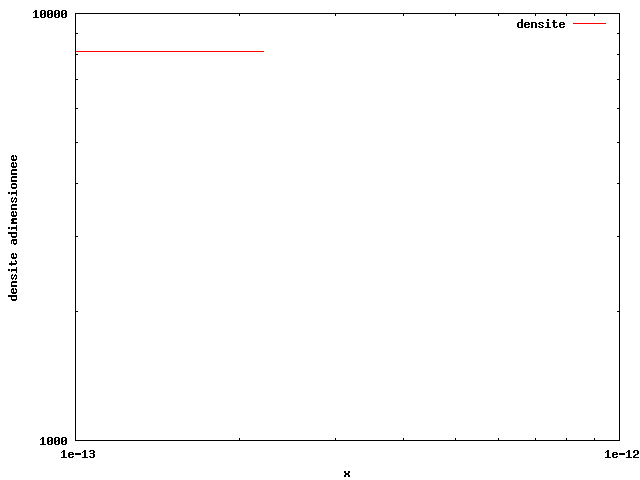
\includegraphics[scale=0.40]{graphe/erreur_king.png}
%			\end{minipage}\hfill
%			\begin{minipage}[b]{0.48\linewidth}
%				\centering 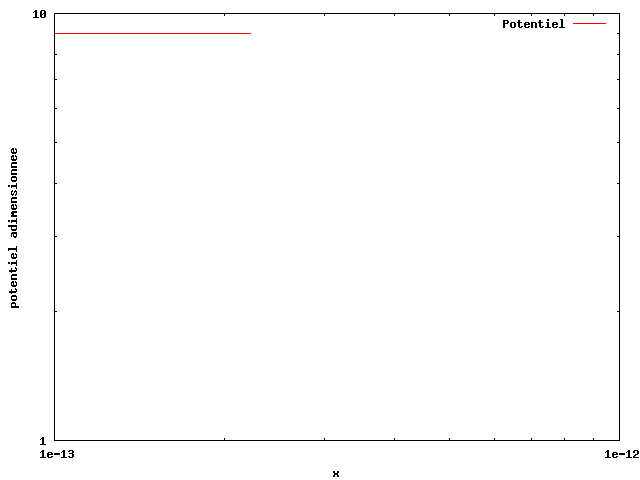
\includegraphics[scale=0.40]{graphe/erreur-pot_king.png}
%			\end{minipage}
%			\caption{Densité et potentiel d'un modèle de \textsc{King} pour les
%			conditions initiales (~au centre~) : $\gamma(0) = \frac{E_l -
%			m\psi(0)}{\sigma^2} = 9$}
%			\label{King_Modele-err}
%	\end{figure}
%	\begin{figure}[ht!]
%			\begin{minipage}[b]{0.40\linewidth}
%				\centering \includegraphics[scale=0.60]{graphe/densite_king.pdf}
%			\end{minipage}\hfill
%			\begin{minipage}[b]{0.48\linewidth}
%				\centering \includegraphics[scale=0.60]{graphe/potentiel_king.pdf}
%			\end{minipage}
%			\caption{Densité et potentiel d'un modèle de \textsc{King} pour les
%			conditions initiales (~au centre~) : $\gamma(0) = \frac{E_l - m\psi(0)}{\sigma^2} = 3$, $\x{\gamma}(0) = 0$}
%			\label{King_Modele}
%	\end{figure}

	\begin{figure}[ht!]
			\begin{minipage}[b]{0.40\linewidth}
				\centering \includegraphics[scale=0.60]{graphe/densite_pluri-king.pdf}
			\end{minipage}\hfill
			\begin{minipage}[b]{0.48\linewidth}
				\centering \includegraphics[scale=0.60]{graphe/densite_pluri_limite-king.pdf}
			\end{minipage}
			\caption{CETTE LEGENDE N4EST PAS SUFFISANTE ! IL FAUT INDIQUER CE QU4EST CETTE FONCTION $\rho(x)$ PARCE CE QUE L4ON CALCULE C4EST $\gamma(x)$.
			Densité d'un modèle de \textsc{King} pour les conditions initiales
			(~au centre~) : $\gamma(0) = 1$ (~courbe rouge~), $5$ (~courbe verte~), $9$ (~courbe bleu~), $14$ (~courbe violette~), $\x{\gamma}(0) = 0$}
			\label{King_Modele-test}
	\end{figure}

	%La figure~\ref{King_Modele-test} montre l'aspect de la densité d'un modèle de \textsc{King} en fonction de $W_0$ et nous indique aussi que ce modèle posséde une structure cœur-halo
	%(~une partie quasiment constante suivi d'une décroissance auto-similaire de pente $\alpha$~).
	%Plus $\phi$ est grand, plus le cœur est dense (~le graphe de droite trace $\rho(x)/\rho(0)$~). Nous pouvons aussi observer que la pente n'est pas la même :
	%elle diminue (~la courbe tend plus vite vers $0$~). Ce constat nous amène à nous poser une question : existe-t-il un
	%lien entre la pente et le rayon du cœur ?
	
	La résolution numérique du système (\ref{sys2dking}) permet d'obtenir la fonction $\gamma(x)$ pour chaque donnée initiale $W_0$. De cette fonction on déduit la densité volumique de masse du système $\rho(x)$ par la relation XXXXXXXXXX. Une sphère de King adimensionnée est donc entièrement définie par le paramètre $W_0$. En échelle logarithmique, sa densité normalisée est très bien approchée sur plus de 5 décades par deux segments de droites : l'un horizontal décrit le c\oe ur de la sphère de densité quasiment constante, l'autre de pente $-\alpha$ décrit un halo autosimilaire entourant le c\oe ur. L'intersection des droites portant ces deux segments est une bonne approximation de ce que l'on pourrait appeler le rayon du c\oe ur de la sphère de King considérée.
		
	Pour les petites valeurs de $W_0$, typiquement $W_0\leq 5$, la sphère de King est essentiellement constituée d'un très large c\oe ur de densité quasiment constante. Par contre dès que  $W_0\geq 15$, le c\oe ur ne renferme plus qu'une faible proportion de la masse du système et la sphère de King est essentiellement constituée d'un halo autosimilaire dont la densité est comparable à celle d'une sphère isotherme. Cette comparaison n'est valide que jusqu’à un certain rayon où la densité de la sphère de King chute violemment  à cause de la troncature introduite par l'énergie de libération.
	Une étude plus fine menée pendant notre stage de M2 montre que les halos des sphères de King sont associés à des profils autosimilaires de pente étagées entre $-5$  et $-2$ lorsque $W_0$ varie de $5$ à $15$.
	
	\begin{figure}[hbt!]
%		\centering \includegraphics[scale=1.00]{../Resol_King/img-king/pente-w0.pdf} %{graphe/evo-coeff_ci.pdf}
		\centering \includegraphics[scale=1.00]{graphe/pente-w0.pdf}%{img-king/pente-w0.pdf} %{graphe/evo-coeff_ci.pdf}
		\caption{Évolution de la pente du halo de la sphère de King en fonction de $W_0$}
		\label{coeff_evo}
	\end{figure}
	
	Une sphère de King définie par une grande valeur de $W_0$ est donc très proche d'une sphère isotherme, sa température est donc vraisemblablement indépendante de la distance au centre. Il est intéressant de préciser cette idée de façon plus quantitative. C'est l'objet de la prochaine section.
	
	\FloatBarrier


%		\newpage
	\section[Relation entre les paramètres]{Relation entre les différents paramètres d'un modèle de \textsc{King}\label{pente-coeff_sec}}
			Nous nous intéressons maintenant à l'existence d'un lien entre le rayon du cœur et la pente
du halo. Il n'y a apparemment aucun moyen de faire ça analytiquement (~en tout cas, je n'ai pas encore trouvé~).
Par contre, lorsque je traçais des graphes, obtenu avec le code abordé ci-dessus,
j'ai remarqué une forte dépendance\footnote{logique~!?!} entre la pente, en $\log-\log$, et $W_0$
(~voir graphe de droite de la figure~\ref{King_Modele-test}~). De même pour le rayon à $10\%$
de l'objet étudié. L'idée que j'ai utilisé pour faire le lien entre les deux quantités a été de
regarder leur comportement en fonction des conditions initiales puis de combiner ensuite les 2
comportements pour obtenir une relation empirique entre ces deux paramètres. %courbe les reliant.

\subsection{Calcul des pentes pour différentes conditions initiales\label{pente-critére}}

	Pour obtenir les pentes, nous traçons dans un diagramme $\log-\log$ la densité, puis, à l'aide
du logiciel \textsc{GNUPlot}\footnote{\url{http://www.gnuplot.info/}} nous ajustons une équation du type $a x+b$ à la partie linéaire de la
courbe, le coefficient $a$ représentant la pente.

	Le problème avec cette méthode, c'est que, pour certaines conditions initiales, il n'y a
presque pas de halo : la densité d'étoile chute brutalement (~voir figure~\ref{ci-pente_1}
page~\pageref{ci-pente_1} en annexe~). Les valeurs des pentes pour des systèmes ayant une énergie de
libération et une énergie minimale très proche, ou une grande dispersion d'énergie, sont donc assez
peu fiables. Cette brusque pente vient de la faible quantité d'énergie à fournir pour faire
s'échapper une ou plusieurs particules du système.

	Le traitement a ensuite été automatisé en considérant que le halo correspond à la zone :
	\begin{align}
		10^{-4} < \dfrac{\rho(r)}{\rho(0)} < 0.1 \label{pente::critere}
	\end{align}

	Pour obtenir les points rouge de la figure~\ref{coeff_evo}, nous avons fait varier $\gamma(0) = W_0 = 1$ à $W_0 = 21$.
	La courbe verte est obtenu en ajustant aux points rouge, et en respectant le critère~\ref{pente::critere}, une équation du type $a e^{b x} + c$. %$a x^2 + b x + c$.
	Les coefficients obtenus sont donnés sur la courbe~\ref{coeff_evo}.
%	\begin{table}[hbt!]
%		\begin{center}
%			\begin{tabular}{|c|c|c|}
%				\hline
%				Coefficient & Valeur & Erreur \\
%				\hline
%				\hline
%				$a$       &         -10.0698      &  $\pm 0.2423$       (~$2.406\%$~) \\
%				\hline
%				$b$       &         0.220152      &  $\pm 0.01075$      (~$4.883\%$~) \\
%				\hline
%				$c$       &         -1.63409      &  $\pm 0.09393$      (~$5.748\%$~) \\
%				$a$       &        $-0.0157022$   &   $\pm 0.002226$ (~$14.18\%$~) \\
%				$b$       &        $0.443128$     &   $\pm 0.03663$  (~$8.266\%$~) \\
%				$c$       &        $-5.33431$     &   $\pm 0.1274$   (~$2.388\%$~) \\
%				\hline
%			\end{tabular}
%		\end{center}
%		\caption{Valeur des coefficients donnée par l'ajustement pour les pentes}
%		\label{pente-fit}
%	\end{table}
	\begin{figure}[hbt!]
%		\centering \includegraphics[scale=1.00]{../Resol_King/img-king/pente-w0.pdf} %{graphe/evo-coeff_ci.pdf}
		\centering \includegraphics[scale=1.00]{graphe/pente-w0.pdf}%{img-king/pente-w0.pdf} %{graphe/evo-coeff_ci.pdf}
		\caption{Évolution des pentes pour différentes conditions initiales}
		\label{coeff_evo}
	\end{figure}

	Il est réconfortant de remarquer sur cette courbe la présence d'une asymptote horizontale autour de $-2$ correspondant à la pente d'une sphère isotherme singulière.
	En effet, pour $W_0 \to \infty$ le modèle de \textsc{King} se rapproche d'une sphère isotherme de rayon infini dont le halo est très proche de celui d'une SIS.
%	\FloatBarrier

\subsection{Calcul du rayon à $10\%$ pour différentes conditions initiales\label{r_10}}

	L'un des paramètres libres les plus utilisés du modèle de \textsc{King} est le rayon du cœur (formule~\ref{r_c}, page~\pageref{r_c}~).
%	Il serait ainsi intéressant de prendre cette valeur et de la tracer en fonction de la condition initiale $W_0$,
%	ce qui nous permettrait ainsi de la relier à la pente.
	Il est donc intéressant de relier les paramètres $r_c$ et $W_0$. Ainsi, en utilisant la relation que nous avons déterminé entre $W_0$ et la pente $\alpha$ du halo, nous obtiendrons une relation entre $r_c$ et $\alpha$

	Mais deux problèmes se posent :
	\begin{enumerate}
		\item de la même manière que dans le paragraphe précédent, la détermination de $r_c$ a un problème : quand
	$W_0$ devient trop grand, le système se \og~dilue~\fg, c'est-à-dire que la différence entre
	cœur et halo est de moins en moins évidente, comme sur la figure~\ref{w_0-5_10}
	page~\pageref{w_0-5_10} (~nous sommes dans le cas d'un amas effondré~),
		\item le programme de résolution qui nous permet d'avoir ces courbes est adimensionné par rapport à ce rayon, rendant ainsi très difficile
			le redimensionnement des résultats et leur comparaison avec les données observationnelles.
	\end{enumerate}

	Pour palier à ce dernier problème, il est possible de prendre, plutôt que le rayon du cœur, le rayon à $10\%$.
%	Le rayon à $10\%$ est le rayon à partir duquel $10\%$ de la masse totale de l'amas se trouve à l'intérieur.
	Il est défini comme :
	\begin{quote}
		Le rayon à $10\%$ du système est atteint lorsque, du centre vers le bord du
		système, la densité a diminué de $10\%$ :
		\begin{align}
			\frac{\rho(x_{10})}{\rho(0)} = 0.1
		\end{align}
	\end{quote}

%	Le rayon à $10\%$ est plus délicat à obtenir.
%	Pour obtenir la figure~\ref{coeur_evo}, nous avons considéré que le rayon à $10\%$ correspondait à la distance pour laquelle la densité
%	ne pouvait plus être considérée comme constante : nous avons placé, à la main, la valeur du
%	rayon au moment où la pente devenait nette\footnote{cette contrainte dépend des gens et n'est donc
%	pas très adapté à ce que nous faisons}.

	Une fois ces valeurs de rayon mesurées, nous avons tracé la courbe rouge de la
	figure~\ref{coeur_evo2} que nous avons ajustée avec la fonction $a e^{b x} + c$ et avons
	obtenu les coefficients indiqués sur la courbe.

%	\begin{table}[hbt!]
%		\begin{center}
%			\begin{tabular}{|c|c|c|}
%				\hline
%				Coefficient & Valeur & Erreur \\
%				\hline
%				\hline
%				$d$       &       $1.86332$      &   $\pm 0.04078$ 	(~$2.189\%$~)\\
%				\hline
%				$e$       &       $-0.635746$    &   $\pm 0.01585$    	(~$2.494\%$~)\\
%				\hline
%				$f$       &       $0.0049355$    &   $\pm 0.003953$     (~$80.1\%$~)\\
%				\hline
%			\end{tabular}
%		\end{center}
%		\caption{Valeur des coefficients donnée par l'ajustement pour les rayons à $10\%$}
%		\label{coeur-fit}
%	\end{table}
%	\begin{figure}[hbt!]
%		\centering \includegraphics[scale=1.00]{graphe/evo-coeur_ci.pdf}
%		\caption{Évolution du rayon à $10\%$ calculé à la main pour différents $W_0$}
%		\label{coeur_evo}
%	\end{figure}

%	\textcolor{red}{\underline{Attention :}} il peut être intéressant de refaire ces courbes en
%	incluant le calcul du rayon à $10\%$ directement dans le code (~selon la définition choisi~).

%	Le calcul a été refait en sortant le rayon à $10\%$ directement du code résolvant les
%	équations. De cette manière, la courbe reste sensiblement la même, et les coefficients ont par contre
%	bien changé, comme nous pouvons le voir sur la courbe~\ref{coeur_evo2}.
	\begin{figure}[hbt!]
		\centering \includegraphics[scale=1.00]{graphe/evo-coeur_ci2.pdf}
		\caption{Évolution du rayon à $10\%$ calculé lors de la résolution numérique pour différents $W_0$}
		\label{coeur_evo2}
	\end{figure}
%	\begin{table}[hbt!]
%		\begin{center}
%			\begin{tabular}{|c|c|c|}
%				\hline
%				Coefficient & Valeur & Erreur \\
%				\hline
%				\hline
%				$d$        &       $7.36877$      &   $\pm 0.2352$       (~$3.191\%$~)\\
%				\hline
%				$e$        &       $-0.633846$    &   $\pm 0.02309$      (~$3.642\%$~)\\
%				\hline
%				$f$        &       $0.0419222$    &   $\pm 0.02291$      (~$54.66\%$~)\\
%				\hline
%			\end{tabular}
%		\end{center}
%		\caption{Valeur des coefficients donnée par l'ajustement pour les rayons à $10\%$
%		(~v2.0~)}
%		\label{coeur-fit2}
%	\end{table}
	\FloatBarrier

\subsection{Lien entre les deux\label{ssec::LinkBetween}}

	Maintenant que nous avons la dépendance des rayons à $10\%$ et des pentes en fonction de la
	condition initiale $W_0$, nous pouvons regarder comment varie la pente en fonction de la
	taille de l'amas. Sur la figure~\ref{coeff-coeur2}, nous avons tracé en vert les données, et
	en rouge la courbe formée par nos deux expressions obtenues par ajustement (~les coefficients
	utilisés sont les mêmes que ceux donnés sur les figures~\ref{coeff_evo} et~\ref{coeur_evo2}~).
%	\begin{figure}[hbt!]
%		\centering \includegraphics[scale=1.00]{graphe/evo-coeff_coeur.pdf}
%		\caption{Évolution de la pente calculé à la main en fonction du rayon à $10\%$}
%		\label{coeff-coeur}
%	\end{figure}

	En supposant que nos ajustements sont valables pour toutes les valeurs possibles de $W_0$,
	nous pouvons tenter d'obtenir une expression analytique reliant nos deux quantités. En
	partant de :
	\begin{align}
		\left\{\begin{array}{l}
			f(W_0) = \alpha = a e^{b W_0} + c \\ %a W_0^2 + b W_0 + c \\
			g(W_0) = x_{10\%} = d e^{e W_0} + f
		\end{array}\right.
	\end{align}
	Et en les combinant :
	\begin{align}
		\Rightarrow e^{e W_0} &= \frac{x_{10\%} - f}{d} \notag\\
				W_0   &= \frac{1}{e}\ln\(\frac{x_{10\%} - f}{d}\) \\
		\Rightarrow \alpha &= a \exp\(\frac{1}{e}\ln\(\frac{x_{10\%} - f}{d}\)\) + c %\frac{a}{e^2}\ln^2\(\frac{x_{10\%} - f}{d}\) +
					%\frac{b}{e}\ln\(\frac{x_{10\%} - f}{d}\) + c \notag \\
%		\intertext{Nous obtenons :}
%		\beta &= a e^{1/e} %\frac{1}{e}\ln\(\frac{x_{10\%} - f}{d}\)\(\frac{a}{e}\ln\(\frac{x_{10\%} - f}{d}\) + b\) + c
	\end{align}

	Cette expression s'ajuste \og~bien~\fg~à la courbe, mais \textsc{GNUPlot} donne des erreurs
	assez élevées.
%	\begin{table}[hbt!]
%		\begin{center}
%			\begin{tabular}{|c|c|c|}
%				\hline
%				Coefficient & Valeur & Erreur \\
%				\hline
%				\hline
%				$q=a/e^2$       &      $-0.0394991$   &   $\pm 0.02115$ (~$53.55\%$~)\\
%				\hline
%				$s=1/d$         &      $0.524033$     &   $\pm 4.538$   (~$865.9\%$~)\\
%				\hline
%				$j=f/d$         &      $0.00254127$   &   $\pm 0.02122$ (~$835.2\%$~)\\
%				\hline
%				$k=b/e$         &      $-0.688944$    &   $\pm 0.8111$  (~$117.7\%$~)\\
%				\hline
%				$l=c$           &      $-5.3267$      &   $\pm 6.127$   (~$115\%$~)\\
%				\hline
%			\end{tabular}
%		\end{center}
%		\caption{Valeur des coefficients donnée par l'ajustement pour les pentes en
%		fonctions des rayons à $10\%$}
%		\label{param-fit}
%	\end{table}
%	Les corrections dans la détermination du rayon à $10\%$ ont amélioré l'ajustement de cette courbe, en plus d'avoir changé l'échelle des $x$. Les changements sont
%	donnés sur la figure~\ref{coeff-coeur2}.
%	\begin{table}[hbt!]
%		\begin{center}
%			\begin{tabular}{|c|c|c|}
%				\hline
%				Coefficient & Valeur & Erreur \\
%				\hline
%				\hline
%				$q$       &       $-0.0526849$    &  $\pm 0.02245$      (~$42.6\%$~)\\
%				\hline
%				$s$       &       $0.211927$      &  $\pm 0.4648$       (~$219.3\%$~)\\
%				\hline
%				$j$       &       $0.0081136$     &  $\pm 0.02144$      (~$264.2\%$~)\\
%				\hline
%				$k$       &       $-0.716362$     &  $\pm 0.1606$       (~$22.42\%$~)\\
%				\hline
%				$l$       &       $-5.01452$      &  $\pm 1.478$        (~$29.47\%$~)\\
%				\hline
%			\end{tabular}
%		\end{center}
%		\caption{Valeur des coefficients donnée par l'ajustement pour les pentes en
%		fonctions des rayons à $10\%$ (~v2.0~)}
%		\label{param-fit2}
%	\end{table}
	\begin{figure}[hbt!]
		\centering \includegraphics[scale=1.00]{graphe/evo-coeff_coeur3.pdf}
		\caption{Évolution de la pente en fonction du rayon à $10\%$}
		\label{coeff-coeur2}
	\end{figure}

%	Ensuite, il est intéressant de comparer les données observationnelle à notre travail. Le problème auquel auquel nous avons fait face est
%	que nous avons adimensionné le problème par rapport au rayon de cœur, qu'il n'est donc pas possible d'obtenir par la résolution numérique.
%	Ce travail n'est donc pas utilisable directement pour une comparaison avec les observations. Par contre, le rayon de cœur est mesurable, comme indiqué dans~\cite{Djo-rc}.
	\FloatBarrier

\subsection{Paramètre de concentration : $c$}
	Le dernier paramètre d'un modèle de \textsc{King} sur lequel nous pouvons jouer est le paramètre de concentration $c$.
	Dans le modèle de King, la concentration s'écrit :
	\begin{align}
		c = \log_{10}\(\frac{R}{r_c}\)
	\end{align}
	avec $R$ la taille du système (~tel que $\rho(R) = 0$~) et $r_c$ le rayon de cœur. Ce paramètre est infini pour la sphère isotherme singulière, comme $W_0$.
	Notons que dans le cas de la SIS $W_0$, $R$ et $c$ sont infini.

	Ce paramètre permet aussi de fixer l'état du système. Trouver une fonction ou une équation permettant de faire le lien entre la concentration et la condition
	initiale $W_0$ nous permettrait de trouver le modèle de King correspondant à un amas (~les paramètres $c$, $r_c$ et $\sigma^2$ le représentant~). Nous avons donc inclus
	dans la résolution des équations un calcul de ce paramètre de concentration. Nous avons ainsi pu obtenir la courbe~\ref{concentre}
	\begin{figure}[hbt!]
		\centering \includegraphics[scale=1.00]{graphe/concentration-king.pdf}
		\caption{Évolution de la concentration avec la condition initiale $W_0$}
		\label{concentre}
	\end{figure}

	Le paramètre de concentration est mesurable pour chaque amas (~en tout cas, c'est un des paramètres du catalogue de \textsc{Harris}~\cite{Harris}~).
	Mais le fait que la courbe ne soit pas bijective nous impose plusieurs modèles pour un seul paramètre de concentration.
	\FloatBarrier


	\section{Température d'un modèle de \King \label{sec::temp}}
		L'une des premières questions que l'on peut se poser, par rapport au modèle précèdent~: le modèle de \King est il isotherme~?

%Dans un premier temps, nous rappelons les expressions des fonctions de distribution et densité pour ce modèle~:
%\begin{align}
%	f_K(E) &= \begin{cases}
%		\rho_0 \(2\pi m\sigma^2\)^{-3/2}\( e^{\frac{E_l-E}{\sigma^2}} - 1\) & \text{si $E < E_l$} \\
%		0 & \text{si $E > E_l$}
%	\end{cases} \\
%	\rho(r) &= \rho_0 \(-\sqrt{\frac{4\phi}{\pi\sigma^2}}\(1 + \frac{ 2\phi }{3\sigma^2}\) + e^{\frac{\phi}{\sigma^2}}\mathrm{erf}\(\sqrt{\phi}/\sigma\)\)
%\end{align}

La température est définit comme étant proportionnelle à la dispersion de vitesse tel que~:
\begin{align}
	T(r) &\propto \dfrac{\int p^2 f_K(E) \vdp}{m^2 \int f_K(E) \vdp} & v^2 = \frac{p^2}{m^2}
\end{align}

\subsection{Évolution de la température avec le rayon}

Le numérateur s'écrit~:
\begin{align}
	\int_0^{p_l} \dfrac{p^2}{m^2} f_K\(E\) \mathrm{d}\vec{p} &= \int_0^{p_l} \dfrac{p^2}{m^2} \rho_0 \(2\pi m\sigma^2\)^{-3/2}\( e^{\frac{E_l-E}{\sigma^2}} - 1\) 4\pi p^2 \ddp \notag \\
	    &= \dfrac{4\pi\rho_0}{\(2\pi m\sigma^2\)^{3/2}}\(\int_0^{p_l} \frac{p^4}{m^2} e^{\frac{E_l-E}{\sigma^2}}\ddp -
	    \int_0^{p_l} \frac{p^4}{m^2}\ddp \) \notag
\intertext{En utilisant $E = \dfrac{p^2}{2m} + m\psi$, et à l'aide d'intégration par partie, il est possible de simplifier plusieurs étapes de l'intégration~:}
	    &= \frac{4\pi\rho_0}{m^2\(2\pi m\sigma^2\)^{3/2}}
	    	\(
			e^{\frac{E_l - m\psi}{\sigma^2}}
			\left[
				3m\sigma^2\int_0^{p_l} p^2 e^{-\frac{p^2}{2m\sigma^2}}\ddp
				- m\sigma^2 p_l^3 e^{-\frac{p_l^2}{2m\sigma^2}}
			\right]
			- \dfrac{p_l^5}{5}
	    	\) \notag \\
	    &= \frac{4\pi\rho_0}{m^2\(2\pi m\sigma^2\)^{3/2}}
		\(
			e^{\frac{E_l - m\psi}{\sigma^2}}
	    		\left[
				  3\(m\sigma^2\)^2 \int_0^{p_l} e^{-\frac{p^2}{2m\sigma^2}} \ddp
				- 3\(m\sigma^2\)^2p_le^{-\frac{p_l^2}{2m\sigma^2}}
			\right. \right. \notag \\
				&\qquad \left.\vphantom{ e^{-\frac{p_l^2}{2m\sigma^2}}}\left.\vphantom{e^{-\frac{p_l^2}{2m\sigma^2}}}
				- m\sigma^2 p_l^3 e^{-\frac{p_l^2}{2m\sigma^2}}
			\right]
	    		- \dfrac{p_l^5}{5}
		\) \notag \\
	    &= \frac{4\pi\rho_0}{m^2\(2\pi m\sigma^2\)^{3/2}}
		\(
			e^{\frac{E_l - m\psi}{\sigma^2}}\(m\sigma^2\)^2
	    		\left[
				  3 \int_0^{p_l} e^{-\frac{p^2}{2m\sigma^2}} \ddp
				- 3p_le^{-\frac{p_l^2}{2m\sigma^2}}
				\(1 + \dfrac{p_l^2}{3m\sigma^2}\)
			\right] \right. \notag \\
	    &\qquad \left.\vphantom{ e^{-\frac{p_l^2}{2m\sigma^2}}}
	    		- \dfrac{p_l^5}{5}
		\) \notag \\
	    &= \frac{4\pi\rho_0}{m^2\(2\pi m\sigma^2\)^{3/2}}
		\(
			e^{\frac{E_l - m\psi}{\sigma^2}}\(m\sigma^2\)^2
	    		\left[
				3 \dfrac{\sqrt{\pi}}{2}\sqrt{2m\sigma^2}\erf\(\dfrac{p_l}{\sqrt{2m\sigma^2}}\)
				- 3p_le^{-\frac{p_l^2}{2m\sigma^2}}
				\(1 + \dfrac{p_l^2}{3m\sigma^2}\)
			\right] \right. \notag \\
	    &\qquad \left.\vphantom{ e^{-\frac{p_l^2}{2m\sigma^2}}}
	    		- \dfrac{p_l^5}{5}
		\) \notag \\
%	    &= \frac{12\pi\rho_0 \sigma^4}{\(2\pi m\sigma^2\)^{3/2}} e^{\frac{E_l - m\psi\(r\)}{\sigma^2}} h\(p_l\)\dr
\intertext{avec $p_l = \sqrt{2m\(E_l - m\psi(r)\)} = \sqrt{2m\phi(r)}$~:}
	    &= \frac{4\pi\rho_0}{m^2\(2\pi m\sigma^2\)^{3/2}}
		\(
			e^{\frac{\phi}{\sigma^2}}\(m\sigma^2\)^2
	    		\left[
				3\dfrac{\sqrt{\pi}}{2} \sqrt{2m\sigma^2}\erf\(\dfrac{\sqrt{2m\phi(r)}}{\sqrt{2m\sigma^2}}\)
			\right. \right. \notag \\
	    &\qquad \left.\vphantom{ e^{-\frac{2m\phi(r)}{2m\sigma^2}}}\left.\vphantom{ e^{-\frac{2m\phi(r)}{2m\sigma^2}}}
			        - 3\sqrt{2m\phi(r)}e^{-\frac{2m\phi(r)}{2m\sigma^2}}
				\(1 + \dfrac{2m\phi(r)}{3m\sigma^2}\)
			\right]
			- \dfrac{\(2m\phi(r)\)^{5/2}}{5}
		\) \notag \\
	    &= \frac{4\pi\rho_0}{m^2\(2\pi m\sigma^2\)^{3/2}}
		\(
			\dfrac{3}{2} \(m\sigma^2\)^2\sqrt{2m\pi\sigma^2}
	    		\left[
				e^{\frac{\phi}{\sigma^2}}\erf\(\sqrt{\dfrac{\phi(r)}{\sigma^2}}\)
			\right. \right. \notag \\
	    &\qquad \left.\vphantom{\(\sqrt{\dfrac{\phi(r)}{\sigma^2}}\) }\left.\vphantom{\(\sqrt{\dfrac{\phi(r)}{\sigma^2}}\)}
				- \sqrt{\dfrac{4\phi(r)}{ \pi\sigma^2}}
				\(1 + \dfrac{2\phi(r)}{3\sigma^2}\)
			\right]
			- \dfrac{\(2m\phi(r)\)^{5/2}}{5}
		\) \notag
\end{align}

La température va alors s'écrire~:
\begin{align}
	T(r) &\propto \frac{4\pi\rho_0}{m^2\(2\pi m\sigma^2\)^{3/2}}
		\(
		\dfrac{
			\dfrac{3}{2} \(m\sigma^2\)^2\sqrt{2m\pi\sigma^2}
	    		\left[
				e^{\frac{\phi}{\sigma^2}}\erf\(\sqrt{\dfrac{\phi(r)}{\sigma^2}}\)
				- \sqrt{\dfrac{4\phi(r)}{ \pi\sigma^2}}
				\(1 + \dfrac{2\phi(r)}{3\sigma^2}\)
			\right]
		}
		{
			\rho_0 \(-\sqrt{\frac{4\phi}{\pi\sigma^2}}\(1 + \frac{ 2\phi }{3\sigma^2}\) + e^{\frac{\phi}{\sigma^2}}\mathrm{erf}\(\sqrt{\phi}/\sigma\)\)
		}
			\right. \notag \\
	    &\qquad \left.
		- \dfrac{
			\(2m\phi(r)\)^{5/2}
		}
		{
			5 \rho_0 \(-\sqrt{\frac{4\phi(r)}{\pi\sigma^2}}\(1 + \frac{ 2\phi(r) }{3\sigma^2}\) + e^{\frac{\phi(r)}{\sigma^2}}\mathrm{erf}\(\sqrt{\phi(r)}/\sigma\)\)
		}
		\) \notag \\
	&\propto \frac{4\pi}{m^2\(2\pi m\sigma^2\)^{3/2}} \(m\sigma^2\)^2
		\(
			\dfrac{3}{2}\sqrt{2m\pi\sigma^2}
		- \dfrac{
			\(2m\phi(r)\)^{5/2} \(m\sigma^2\)^{-2}
		}
		{
			5 \(-\sqrt{\frac{4\phi(r)}{\pi\sigma^2}}\(1 + \frac{ 2\phi(r) }{3\sigma^2}\) + e^{\frac{\phi(r)}{\sigma^2}}\mathrm{erf}\(\sqrt{\phi(r)}/\sigma\)\)
		}
		\) \notag \\
	&\propto \sqrt{\dfrac{2\sigma^2}{m^3\pi}}							%\frac{4\pi}{m^2\(2\pi m\sigma^2\)^{3/2}} \(m\sigma^2\)^2
		\(
			\dfrac{3}{2}\sqrt{2m\pi\sigma^2}
		- \dfrac{
			\(2m\phi(r)\)^{5/2} \(m\sigma^2\)^{-2}
		}
		{
			5 \(-\sqrt{\frac{4\phi(r)}{\pi\sigma^2}}\(1 + \frac{ 2\phi(r) }{3\sigma^2}\) + e^{\frac{\phi(r)}{\sigma^2}}\mathrm{erf}\(\sqrt{\phi(r)}/\sigma\)\)
		}
		\)
\end{align}
Nous obtenons alors une expression de la température qui n'est pas analytique. Pour obtenir la température, nous reprenons le noyau développé autour
du modèle de \King pendant le stage, puis nous appliquons la formule obtenue.
Les courbes obtenues sont données tracé sur les graphes~\ref{courbe::Temp}.
\begin{figure}[H]
	\begin{minipage}[b]{0.40\linewidth}
		\centering \includegraphics[scale=0.60]{theorie/graphe/temperature_0-997636.pdf}
	\end{minipage}\hfill
	\begin{minipage}[b]{0.48\linewidth}
		\centering \includegraphics[scale=0.60]{theorie/graphe/temperature_3-98531.pdf}
	\end{minipage}
	\centering \includegraphics[scale=0.60]{theorie/graphe/temperature_11-1096.pdf}
	\caption{Courbes de température pour différents $W_0$\label{courbe::Temp}}
\end{figure}
%\FloatBarrier

Toutes ces courbes sont normalisées par rapport à la température centrale donnée par~:
\begin{align}
	T(0) &\propto \sqrt{\dfrac{2\sigma^2}{m^3\pi}}								%\frac{4\pi\rho_0}{m^2\(2\pi m\sigma^2\)^{3/2}} \(m\sigma^2\)^2
		\(
			\dfrac{3}{2}\sqrt{2m\pi\sigma^2}
		- \dfrac{
			\(2m\phi(0)\)^{5/2} \(m\sigma^2\)^{-2}
		}
		{
			5 \(-\sqrt{\frac{4\phi(0)}{\pi\sigma^2}}\(1 + \frac{ 2\phi(0) }{3\sigma^2}\) +
			e^{\frac{\phi(0)}{\sigma^2}}\mathrm{erf}\(\sqrt{\phi(0)}/\sigma\)\)
		}
		\) \notag \\
	   &\propto \sqrt{\dfrac{2\sigma^2}{m^3\pi}}								%\frac{4\pi\rho_0}{m^2\(2\pi m\sigma^2\)^{3/2}} \(m\sigma^2\)^2
		\(
			\dfrac{3}{2}\sqrt{2m\pi\sigma^2}
		- \dfrac{
			\(2m\sigma^2W_0\)^{5/2} \(m\sigma^2\)^{-2}
		}
		{
			5 \(-\sqrt{\frac{4W_0}{\pi}}\(1 + \frac{ 2W_0 }{3}\) +
			e^{W_0}\mathrm{erf}\(\sqrt{W_0}\)\)
		}
		\)
\end{align}
%\FloatBarrier

\subsection{Température moyenne d'un modèle de \King}
\label{Calc::Temp}

Au vu de ces courbes, nous pouvons considérer que la sphère de \King est bien isotherme. Il est alors possible de déterminer une température moyenne~:
\begin{align}
%	T_{\mathrm{moy}} &= \dfrac{\displaystyle{\int}_0^R 4\pi r^2 T(r) f_K(E) \dr}{\displaystyle{\int}_0^R 4\pi r^2 \dr} \\
%			 &= \dfrac{\displaystyle{\int}_0^R r^2 T(r) \rho_0 \(2\pi m\sigma^2\)^{-3/2}\( e^{\frac{E_l-E}{\sigma^2}} - 1\)}
%			 	  {\displaystyle{\int}_0^R r^2      \rho_0 \(2\pi m\sigma^2\)^{-3/2}\( e^{\frac{E_l-E}{\sigma^2}} - 1\)}
T_{\mathrm{moy}} &= \dfrac{\displaystyle{\int}\displaystyle{\int}\frac{p^2}{m^2}f_K(E)\vdp\vdr}{\displaystyle{\int}\displaystyle{\int}f_K(E)\vdp\vdr} \notag \\ %\int_0^R 4\pi r^2 T(r) \dr \\
	    &= \frac{4\pi\rho_0}{Mm^2\(2\pi m\sigma^2\)^{3/2}}
		    \displaystyle{\int}_0^R 4\pi r^2\(
			\dfrac{3}{2} \(m\sigma^2\)^2\sqrt{2m\pi\sigma^2}
	    		\left[
				e^{\frac{\phi}{\sigma^2}}\erf\(\sqrt{\dfrac{\phi(r)}{\sigma^2}}\)
			\right. \right. \notag \\
	    &\qquad \left.\vphantom{\(\sqrt{\dfrac{\phi(r)}{\sigma^2}}\) }\left.\vphantom{\(\sqrt{\dfrac{\phi(r)}{\sigma^2}}\)}
				- \sqrt{\dfrac{4\phi(r)}{ \pi\sigma^2}}
				\(1 + \dfrac{2\phi(r)}{3\sigma^2}\)
			\right]
			- \dfrac{\(2m\phi(r)\)^{5/2}}{5}
		\) \dr \notag \\
	    &= \frac{4\pi}{Mm^2\(2\pi m\sigma^2\)^{3/2}}
		    \(
			\dfrac{3}{2} \(m\sigma^2\)^2\sqrt{2m\pi\sigma^2}
	    		\displaystyle{\int}_0^R 4\pi r^2 \rho_0\left[
				e^{\frac{\phi}{\sigma^2}}\erf\(\sqrt{\dfrac{\phi(r)}{\sigma^2}}\)
			\right. \right. \notag \\
	    &\qquad \left.\vphantom{\(\sqrt{\dfrac{\phi(r)}{\sigma^2}}\) }\left.\vphantom{\(\sqrt{\dfrac{\phi(r)}{\sigma^2}}\)}
				- \sqrt{\dfrac{4\phi(r)}{ \pi\sigma^2}}
				\(1 + \dfrac{2\phi(r)}{3\sigma^2}\)
			\right] \dr
			-\displaystyle{\int}_0^R 4\pi r^2 \rho_0 \dfrac{\(2m\phi(r)\)^{5/2}}{5} \dr
		\) \notag \\
	    &= \frac{4\pi}{Mm^2\(2\pi m\sigma^2\)^{3/2}}
		    \(
			\dfrac{3}{2} \(m\sigma^2\)^2\sqrt{2m\pi\sigma^2}
	    		\displaystyle{\int}_0^R 4\pi r^2 \rho(r) \dr
			-\displaystyle{\int}_0^R 4\pi r^2 \rho_0 \dfrac{\(2m\phi(r)\)^{5/2}}{5} \dr
		\) \notag \\
	    &= \frac{4\pi}{Mm^2\(2\pi m\sigma^2\)^{3/2}}
		    \(
			\dfrac{3}{2} \(m\sigma^2\)^2\sqrt{2m\pi\sigma^2}
	    		M
			-\displaystyle{\int}_0^R 4\pi r^2 \rho_0 \dfrac{\(2m\phi(r)\)^{5/2}}{5} \dr
		\) \notag \\
	    &= \frac{4\pi}{Mm^2\(2\pi m\sigma^2\)^{3/2}}
			\dfrac{3}{2} \(m\sigma^2\)^2\sqrt{2m\pi\sigma^2}
	    		M
			-\frac{4\pi}{Mm^2\(2\pi m\sigma^2\)^{3/2}}\displaystyle{\int}_0^R 4\pi r^2 \rho_0 \dfrac{\(2m\phi(r)\)^{5/2}}{5}\dr \notag \\
	    &= \frac{3\sigma^2}{m} - \frac{4\pi}{Mm^2\(2\pi m\sigma^2\)^{3/2}}\displaystyle{\int}_0^R 4\pi r^2 \rho_0
	    \dfrac{\(2m\phi(r)\)^{5/2}}{5}\dr \notag \\
	    &= \frac{3\sigma^2}{m} - \frac{32\pi^2\rho_0}{5 M m\(\pi \sigma^2\)^{3/2}}\displaystyle{\int}_0^R r^2 \(\phi(r)\)^{5/2}\dr
\end{align}
\begin{figure}[h!]
	\centering \includegraphics[width=1.00\textwidth]{theorie/graphe/Temperature_centre-moyenne.pdf}
	\caption{Températures maximums et moyennes en fonction de $W_0$\label{courbe::Moy}}
\end{figure}
La courbe~\ref{courbe::Moy} représente la variation des températures moyennes et centrales pour notre amas. Sur la courbe verte représentant la
température moyenne, un régime assez étrange commence à apparaître vers les $W_0$. Ce nouveau régime peut avoir 2 source possible~:
\begin{enumerate}
	\item une instabilité numérique apparaissant à cause de valeurs trop importante ou trop faible (~présence de \textsc{Not A Number} dans le
		fichier de donnée~),
	\item le $W_0$ à une valeur maximum au-delà de laquelle les équations ne sont plus valable.
\end{enumerate}
La première chose à faire dans ce cas est de tracer le maximum de profil de densité pour ces valeurs, de même il va falloir étudier la variation de
$\rho(r=0)$ en fonction de $W_0$.

Il est utile de rappeler que le but de ces travaux est de trouver les quantités à utiliser pour tracer un diagramme d'énergie similaire à celui de la
sphère isotherme en boîte, et ceci afin d'en étudier la stabilité.

Pour ceci nous avons d'avoir chercher à vérifier que le modèle est isotherme, ce qui est vérifié par les courbes~\ref{courbe::Temp}. Puis nous devions
savoir si la quantités à utiliser comme température est la température moyenne ou la température centrale. Ce dernier point est assez délicat
\FloatBarrier



	\section{Synthèse}
		Nous avons maintenant étudié trois modèles pouvant décrire l'état d'équilibre d'un amas d'étoile:
\begin{description}
	\item[La sphère isotherme] (\textsc{si}) est un modèle thermodynamique étudié sur un support spatial infini. Ce modèle avait l'avantage de posséder une solution analytique,
		mais cette solution possède, comme nous l'avons montré, une masse infinie.
	\item[La sphère isotherme en boîte] (\textsc{sib}) est une variante du modèle de \textsc{si} avec une extension
		finie. Grâce à ce modèle, nous avons appris que l'étude de la stabilité était pilotée par un seul paramètre important:
		le contraste de densité $\R_c$.
	\item[Le modèle de King] est lui aussi une variante de \textsc{si}, mais avec une coupure plus physique, effectuée après coup. Il nous a permis de montrer que l'évolution
		de la pente du halo, et donc du contraste de densité, pouvait être liée à un seul paramètre: $W_0$.
		Une étude de sa température nous a confirmé que ce modèle pouvait être considéré comme isotherme dès lors qu'il est un peu évolué
		($W_0 > 5$) et qu'il correspond à un amas globulaire (pente du halo supérieur à $-5$).
		% Cette évolution peut-être décrite par une équation de la forme $\alpha = a e^{b W_0} + c$.
\end{description}


\chapter{Étude de quelques amas}
	\minitoc
	\section{Introduction}
			Nous avons dénombré environ 150 amas globulaires dans notre galaxie. Sur ces amas, $20\%$ ont un cœur effondré. %, mais pas les $80\%$ restants.
	Depuis une centaine d'année, des astrophysiciens --~tel \textsc{Chandrasekhar}, \textsc{King}, ...~--
	tentent d'expliquer à l'aide de différents modèles les propriétés observées de ces objets.
	Nous avons étudié dans les chapitres précédents deux \og grands modèles \fg~décrivant ces états d'équilibres,
	mais le point qui intéresse plus spécialement les physiciens est l'évolution des amas : comment en sont-ils
	arrivés là et que pourraient-ils devenir ?

	Du fait de nos développements théoriques dans les chapitres précédents, nous avons la possibilité de lier
	$W_0$ à la pente de la densité d'un modéle de \textsc{King},  modèle le plus utilisé lorsqu'il s'agit d'ajuster des données.
%	Dans~\cite{King-1966AJ}, Ivan R. \textsc{King} donne quelques explications sur pourquoi le modéle de la sphère isotherme singuliére
%	n'est pas utilisé et l'intérêt d'utiliser des modéles limité spatialement.

	Sur les graphes~\ref{effondre} et~\ref{pas_effondre} nous pouvons voir la courbe de densité
	d'un amas, respectivement, au cœur effondré et au cœur ne l'étant.
%	Le scénario utilisé ici, et qui sera étudié plus en détaille lors des simulations numériques, consiste en un \og~effeuillage~\fg progressif de l'amas : sa présence
%	dans le potentiel galactique lui fait perdre, petit à petit, des étoiles. Cette perte d'étoile va faire rétrécir le cœur de l'amas selon le processus mentionné dans
%	la section~\ref{petit_scenar} (~dû à la capacité calorifique négative~).
%	Une perte d'étoile trop importante entraînant ainsi un effondrement.
%	Le scénario ainsi évoqué peut-être résumé, de façon schématique, comme sur le schéma~\ref{schema-effondrement}.
%	Les études développées dans les chapitres précédents nous amènent à considérer que le système se comporte comme ayant un cœur et un halo bien distinct, l'un
%	caractérisé par sa densité constante, l'autre par la pente avec laquelle décroit la dite densité.
	Les études précédentes nous permettent de considérer que les objets étudiés possèdent une structure cœur-halo. Le cœur est la région dans laquelle la densité est constante ; le halo est la région dans laquelle la densité
	décroit selon une loi en $r^{-\alpha}$, la constante $\alpha$ étant appelée la pente du halo.

	\begin{figure}[ht!]
		\begin{minipage}[b]{0.48\linewidth}
			\begin{center}
%				\begin{gnuplot}[terminal=pdf,scale=0.50]
%					set xlabel "Distance au centre"
%					set ylabel "Densitee adimensionee et normalisee"
%					set title "Profil de densite de NGC 1904"
%					plot 'NGC1904.res' u 1:2 w p title "Densite de NGC 1904", '' u 1:2 smooth bezier not
%				\end{gnuplot}
%					plot '../Amas/res/NGC1904.res' u 1:2 w p title "Densite de NGC 1904", '' u 1:2 smooth bezier not
%				\includegraphics[scale=0.7]{graphe/NGC1904-2.pdf}
				\includegraphics[width=1.0\linewidth]{graphe/NGC1904-2.pdf}
				\caption{\footnotesize{Profil non effondré : \mbox{NGC 1904}} \label{pas_effondre}}
%				\begin{figure}[h]
%					\includegraphics[scale=0.5]{graphe/NGC1904.pdf}
%					\caption{Profil non effondré : NGC 1904 \label{effondre}}
%				\end{figure}
			\end{center}
		\end{minipage}\hfill
		\begin{minipage}[b]{0.48\linewidth}
			\begin{center}
%				\begin{gnuplot}[terminal=pdf,scale=0.50]
%					set xlabel "Distance au centre"
%					set ylabel "Densitee adimensionee et normalisee"
%					set title "Profil de densite de Terzan 2"
%					plot 'Terzan_2.res' u 1:(($2>2)?0:$2) w p title "Densite de Terzan 2", '' u 1:2 smooth bezier not
%				\end{gnuplot}
%					plot '../Amas/res/Terzan_2.res' u 1:(($2>2)?0:$2) w p title "Densite de Terzan 2", '' u 1:2 smooth bezier not
%				\includegraphics[scale=0.7]{graphe/Terzan_2.pdf}
				\includegraphics[width=1.0\linewidth]{graphe/Terzan_2.pdf}
				\caption{\footnotesize{Profil effondré : \mbox{Terzan 2}} \label{effondre}}
%				\begin{figure}[h]
%					\includegraphics[scale=0.5]{graphe/NGC1904.pdf}
%					\caption{Profil effondré : NGC 5946 \label{pas_effondre}}
%				\end{figure}
			\end{center}
		\end{minipage}
%		\caption{Exemple de profil de densité}
	\end{figure}
\normalsize


	\section[Lien]{Lien entre données et paramètres\label{amas}}
%			Comme nous l'avons déjà dit dans la section~\ref{r_10}, les travaux que nous avons effectué
%			sur le rayon de cœur ne sont pas exploitable en l'état à cause de l'adimensionnement du
%			problème. Par contre, l'utilisation de l'équation d'ajustement du graphe~\ref{coeff_evo}
%			pour une valeur de la pente en fonction de $W_0$ nous permet déjà d'obtenir
%			une solution pour chaque amas où le calcul de cette pente est possible.
%			Pour les autres paramètres comme le rayon de cœur, le problème reste entier.
		\subsection{Préliminaire}
%	Ce qui va nous intéresser ici, c'est de pouvoir lier à chaque étape d'évolution d'un amas, et donc à son âge,
%	une pente.
	Notre objectif est de trouver une relation entre l'âge d'un amas et la pente de son halo.
	%Nous avons donc besoin d'une relation entre cette quantité et l'âge de l'amas, si une telle relation existe.
	Nous avons alors utilisé le temps de relaxation donné dans le catalogue de \textsc{Harris}~\cite{Harris}.
	Pour obtenir les pentes des amas, nous avons utilisé les relevés observationnels~\cite{Trager-graphe}. % (~les données ainsi obtenues et utilisées sont dans la table~\ref{pente-Tc:BSP}~).
	Nous avons commencé par calculer les pentes directement sur les courbes avec un double décimètre, n'ayant alors pas pu obtenir les données correspondant aux graphiques.
	Après avoir tracé la pente mesurée en fonction du temps de relaxation à 2 corps, nous avons ajusté la
	courbe ainsi obtenue par une droite d'équation $ \alpha = \mathrm{pente} = a \log_{10}(T_c) + b$ (~graphe~\ref{Pente-lin}~).
	\begin{figure}[hbt!]
		\centering \includegraphics[scale=0.9]{graphe/Pente-Tc.pdf}
		\caption{Évolution des pentes pour différents âges}
		\label{Pente-lin}
	\end{figure}
%	\begin{table}[hbt!]
%		\begin{center}
%			\begin{tabular}{|c|c|c|}
%				\hline
%				Coefficient & Valeur & Erreur \\
%				\hline
%				\hline
%				$a$       &        $-1.19506$   &   $\pm 0.1576$ (~$13.19\%$~) \\
%				\hline
%				$b$       &        $2.52082$     &   $\pm 1.213$   (~$48.11\%$~) \\
%				\hline
%			\end{tabular}
%		\end{center}
%		\caption{Valeur des coefficients donnée par l'ajustement pour les pentes}
%		\label{pente-lin-coeff}
%	\end{table}

	Cette approche indiquant clairement une relation linéaire entre ces deux paramètres, nous avons décidé d'entreprendre une démarche plus globale et automatique.
	Pour commencer, nous avons donc récupéré les données auprès des auteurs de l'article sur~\cite{TragerTable}. Nous nous sommes alors confronté au problème des unités.

\subsection{Retraitement}
	Le graphique~\ref{Pente-lin} a été obtenu en utilisant~\cite{Trager-graphe} avec ses unités. % (~les données permettant de retracer, nous les avons finalement trouvé,
%	les graphiques de cet article sont données dans~\cite{TragerTable}~).
	La pente donnée ici n'est donc pas la pente de la densité, mais de la brillance de surface de l'objet en fonction d'un rayon en seconde d'arc.
	Le premier traitement à effectuer consiste donc à transformer cette brillance de surface par arc seconde carrée en une densité (~kilogramme par kilomètre au cube~).

	Une définition de cette brillance de surface, telle qu'elle semble avoir été utilisée, peut-être trouvé dans~\cite{SBP}.
	Comme indiqué dans ce texte, la brillance de surface va s'écrire :
	\begin{align}
		\mu_V = \mu_{\mathrm{ref}} - 2.5 \log_{10}\(\frac{f/\Omega}{f_{\mathrm{ref}}/\Omega_{\mathrm{ref}}}\)
		\label{mu_V}
	\end{align}
	avec $\Omega$ l'angle solide, exprimé en seconde d'arc au carrée, sous lequel nous voyons l'objet.
%	\begin{align}
%		\mu_V = m_V - 2.5 \log_{10}\(\frac{(1\mathrm{"})^2}{\Omega}\)
%		\label{mu-astuce}
%	\end{align}
%	avec $m_V$ la magnitude apparente de l'objet sur une seconde d'arc au carrée.

	Cette définition rappelle celle de~\cite{Trager-graphe}, section~3.2.3 :
	\begin{align}
		\mu = -2.5 \log\(\frac{10^{-0.4 m_2} - 10^{-0.4 m_1}}{\pi \(r_2^2 - r_1^2\)}\)
		\label{Trager-eq}
	\end{align}
%	où ils prendraient comme référence les points autour de celui considéré (~ou quelque chose comme ça~),
	$m_i$ étant la magnitude en un point de l'objet et $r_i$ le rayon en seconde d'arc pour ce point.
	Par conséquent, les unités de $\mu$ sont un flux par arc seconde carrée en échelle logarithmique :
	\begin{enumerate}
		\item $10^{-0.4 m_i}$ est proportionnel à un flux, % (~ou au rapport d'un flux par rapport à un flux de référence !?!~),
		\item $r_i$ est le rayon de l'objet au point $i$ en seconde d'arc,
		\item[$\Rightarrow$] nous avons donc bien notre flux par seconde d'arc au carrée.
	\end{enumerate}
	Pour pouvoir revenir aux quantités que nous cherchons, il va falloir calculer un peu :
	\begin{align}
		\mu = -2.5 \log\(\frac{10^{-0.4 m_2} - 10^{-0.4 m_1}}{\pi \(r_2^2 - r_1^2\)}\) &\equiv -2.5 \log\(\frac{F}{\pi \(r_2^2 - r_1^2\)}\) \text{avec $F$ le flux}\notag \\
		\intertext{par rapport à toute la documentation que j'ai trouvé, le $\log$ correspond ici à $\log_{10}$ et non à $\ln$.}
		\Rightarrow \frac{F}{\pi \(r_2^2 - r_1^2\)} &= 10^{-\mu/2.5} \label{F--mu} \\
		\intertext{Grâce à~\cite{McL}, nous avons les rapports masse luminosité :}
		\Upsilon &= \frac{M}{L} \label{M/L}\\
		\intertext{or}
		F &= \frac{L}{4\pi D^2} \label{def-F}\\
		\intertext{avec $D$ la distance soleil--amas. D'où}
		\frac{L}{4 \pi^2 \(r_2^2 - r_1^2\) D^2} &= \frac{M}{4 \pi^2 \Upsilon \(r_2^2 - r_1^2\) D^2} = 10^{-\mu/2.5} \notag \\
		\intertext{en combinant~\ref{F--mu}, \ref{M/L} et~\ref{def-F}.}
		\Rightarrow \frac{M}{4\pi \(r_2^2 - r_1^2\)} &= \pi\Upsilon D^2 10^{-\mu/2.5} \notag \\
		\intertext{Mais $r_2^2 - r_1^2 \propto r_i^2$ doit être converti en mètre :}
		%r_2^2 - r_1^2 &\propto r_i^2 \Rightarrow \(D \tan(r_i)\)^2 \varpropto \(D r_i\)^2 \notag \\
		\Rightarrow \frac{M}{4\pi \(D \tan(r_i/3600)\)^2} &= \pi\Upsilon D^2 10^{-\mu/2.5} \label{M-don}
	\end{align}
	Normalement, nous avons maintenant une masse surfacique donnée par~\ref{M-don}.
%	mais, étonnamment, la conversion de seconde d'arc à mètre n'a fait paraître
%	aucun facteur numérique !!! J'ai peut-être un peu trop truandé.

	Les rapports masse-luminosité peuvent être trouvés dans~\cite{McL}, mais cette article ne contient que 40 des 140 amas de notre galaxie.
%	mais il n'y a qu'une quarantaine de rapport comparé à notre échantillon d'environ 140 amas.
	Par contre, il est aisé de remarquer que ces rapports sont
	en moyenne très peu différents de la valeur $\Upsilon = 2$ avec une valeur minimum de $1.87$ pour NGC 4147 et une valeur maximum de
	$2.66$ pour NGC 6441. Dans la suite, nous prendrons donc $\Upsilon = 2$.
%	Nous avons alors utilisé les données du catalogue pour redimensionner le tout, mais pour passer à la densité, nous avons besoin du rapport masse
%	sur luminosité de l'amas qui peut-être trouvé dans~\cite{McL}.
%	Cet article ne donne qu'une quarantaine d'amas sur les 150 de notre galaxie, mais les valeurs de ces rapports étant compris entre $1.87$ pour NGC 4147
%	(~et quelques autres~) et $2.66$ pour NGC 6441, et tournant surtout autour de $2$, nous pouvons supposer que ces rapports sont les mêmes pour chaque amas et
%	valent $\Upsilon = \frac{M}{L} = 2$.
%	Selon~\cite{Trager-graphe}, nous avons donc :
%	\begin{align}
%		\mu_V &\propto \text{Flux par $m^{-2}$} = \frac{L}{4\pi D^2} \\
%		\intertext{or}
%		L &= \frac{M}{\Upsilon} \notag \\
%		\intertext{donc}
%		\mu_V &= \frac{M}{4\pi D^2 \Upsilon} \notag \\
%		M &= \Upsilon \mu_V 4\pi D^2
%	\end{align}
%	avec $D$ la distance entre nous et l'amas. Nous pouvons supposer que cette distance est la même quelque soit l'étoile considéré dans l'amas
%	(~$D_{min} = 3000\mathrm{pc} \gg R_{amas} \approx 10\mathrm{pc}$~).

%	Du fait des rapports masse-luminosité manquant, notre échantillon d'une quarantaine d'amas est passé à seulement 12 amas.

\subsection{Résultat}
	Le calcul de pente a été refait en utilisant : les données de l'article~\cite{TragerTable}, le traitement décrit ci-dessus, et le critère donné dans la section~\ref{pente-critére}.
	Nous obtenons alors le graphique~\ref{Pente-lin_dim}, l'ajustement utilisant la fonction
	$f(T_c) = a \log(T_c) + b$ (~les coefficients ont été donnés dans la table~\ref{pente-lin-coeff_dim}~).
	Nous avons donc maintenant une relation linéaire entre l'âge de l'amas et la pente du halo.

	\begin{figure}[hbt!]
%		\centering \includegraphics[scale=0.9]{../Amas/Graphe_Rapport/pente-Tc.pdf}
		\centering \includegraphics[scale=0.9]{graphe/pente-Tc.pdf}
		\caption{Évolution des pentes pour différents âges}
		\label{Pente-lin_dim}
	\end{figure}
	\begin{table}[hbt!]
		\begin{center}
			\begin{tabular}{|c|c|}%c|}
				\hline
				Coefficient & Valeur \\ %& Erreur \\
				\hline
				\hline
				$a$       &         $-2.3341$   \\ %&    $\pm 0.2075$      (~$32.34\%$~) \\
				\hline
				$b$       &         $16.913$   \\  %&    $\pm 1.638$       (~$199.5\%$~) \\
				\hline
			\end{tabular}
		\end{center}
		\caption{Valeurs des coefficients donnée par l'ajustement pour les pentes pour le temps de croisement}
		\label{pente-lin-coeff_dim}
	\end{table}

	Nous avons également utilisé le catalogue de \textsc{Harris} pour obtenir le lien entre la pente du halo et le temps dynamique
	grâce à l'équation~\ref{Td:sig}. Nous obtenons alors le graphique~\ref{Pente-Td-lin}.
	\begin{figure}[hbt!]
%		\centering \includegraphics[scale=0.9]{../Amas/Graphe_Rapport/pente-Td.pdf}
		\centering \includegraphics[scale=0.9]{graphe/pente-Td.pdf}
		\caption{Évolution des pentes pour différents âges dynamiques}
		\label{Pente-Td-lin}
	\end{figure}
	\begin{table}[hbt!]
		\begin{center}
			\begin{tabular}{|c|c|}%c|}
				\hline
				Coefficient & Valeur \\ %& Erreur \\
				\hline
				\hline
				$a$       &        $-1.6567$   \\ %&   $\pm 0.6523$      (~$278.9\%$~) \\
				\hline
				$b$       &        $1.8927$     \\ %&   $\pm 2.825$       (~$88.57\%$~) \\
				\hline
			\end{tabular}
		\end{center}
		\caption{Valeurs des coefficients donnée par l'ajustement pour les pentes pour le temps dynamique}
		\label{pente-Td-lin-coeff}
	\end{table}

	Sur la figure~\ref{Pente-lin_dim}, nous pouvons noter la présence de 2 points avec des pentes inférieures à $-10$. Ces points correspondent aux amas NGC 5024 et NGC 5139
	(~leurs densités sont donnée en annexe, page~\pageref{Graphe-bofbof}~) pour lesquelles la détermination des pentes n'a pas été très concluante.
	\FloatBarrier



	\section{Interprétation}
		Nous avons maintenant une équation liant la valeur de la pente au temps de relaxation : $ \mathrm{pente} = \alpha = d * \log_{10}(T_c) + e $ (~coefficients table~\ref{pente-lin-coeff_dim}~)
et une autre liant la pente à $W_0$ : $ \alpha = a e^{ b W_0 } + c $.
En combinant ces deux équations, nous pouvons obtenir une relation entre le temps de
relaxation et $W_0$ :
\begin{align}
	\mathrm{pente} &= d \log_{10}(T_c) + e = a e^{b W_0} + c \notag \\
	\Rightarrow W_0 &= \frac{1}{b} \ln\( \frac{d \log_{10}(T_c) + e - c}{a} \) \label{Tc:W0->fct}
\end{align}
avec :
\begin{table}[h!]
	\begin{center}
		\begin{tabular}{|c|r|}
			\hline
			Coefficient	&	Valeur \\
			\hline
			\hline
			$a$		&	$ -10.0698 $ \\
				\hline
			$b$		&	$ 0.220152 $ \\
			\hline
			$c$		&	$ -1.53409 $ \\
			\hline
			$d$		&	$ -2.3341 $ \\
			\hline
			$e$		&	$ 16.913 $ \\
			\hline
		\end{tabular}
	\end{center}
\end{table}

Le comportement que nous avions observé en étudiant le modèle de \textsc{King}, à savoir une évolution de la pente avec $W_0$, se retrouve avec l'âge de notre amas. Ce qui nous a permis de relier
l'âge et $W_0$.
Il nous reste à interpreter ces résultats, ce que nous allons faire dans la section suivante.


	\section{Petit Scénario\label{petit_scenar}}
%			Le petit scénario évoqué dans la section~\ref{petit_scenar} donne déjà un élément de réponse quant à leurs
%			évolutions.
%			C'est ce petit scénario que nous allons comparer aux données.
%			Mais d'abord analysons-le pour trouver quels observables utiliser.
%			Nous avons vu dans ce scénario que le rayon du coeur diminuait quand sa température augmentait : pour faire
%			augmenter cette température, il faut augmenter le potentiel $\psi < 0$ et donc retirer de la matiére.
%			Quand cette perte de matiére (~du cœur ou du halo~) devient trop importante, il y a un effondrement.
%			Le processus d'effondrement pourrait donc être lié à un processus \og~d'effeuillage~\fg (~perte d'étoiles
%			par l'amas dû, par exemple, à sa présence dans le potentiel galactique~).
%			Ainsi, si il y a effondrement, le rayon de cœur de l'amas va diminuer, et le halo va lui aussi voir son
%			rayon diminuer, mais, la densité du cœur augmentant, la pente (~pour une densité tracé en $\log-\log$~)
%			avec laquelle il diminue va elle aussi changer.
		%Nous avons vu que les courbes~\ref{King_Modele-test} peuvent être divisées en deux parties : l'une, caractérisée par une densité constante, constituant un cœur, et l'autre constituant un halo.
%Nous allons donc considérer un amas d'étoile composé d'un cœur dense et d'un halo.
%Le halo a peu de gravité et se comporte comme un gaz parfait.
%Le comportement observé dans notre étude est résumé sur le schéma~\ref{schema-effondrement} :
%
	\begin{figure}[ht!]
		\begin{minipage}[b]{0.20\linewidth}
			\begin{center}
				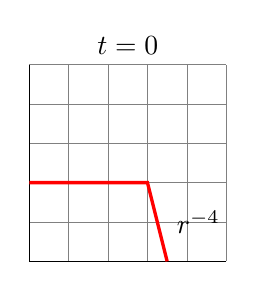
\begin{tikzpicture}
%					Tracé de la grille :
					\draw[step=.5cm,gray,very thin] (0,0) grid (2.5,2.5);
%					Tracé des axes :
					\draw (0,0) -- (0,2.5);
					\draw (0,0) -- (2.5,0);
%					Tracé du graphe :
					\draw[red,very thick] (0,1.0) -- (1.5,1.0) -- (1.75,0);
%					\draw[red,very thick] (1.5,1.0) -- (1.75,0);
					\draw (1.75,0.5) node[right]{$r^{-4}$};
					\draw (1.25,2.5) node[above]{$t = 0$};
				\end{tikzpicture}
			\end{center}
		\end{minipage}\hfill
		\begin{minipage}[b]{0.20\linewidth}
			\begin{center}
				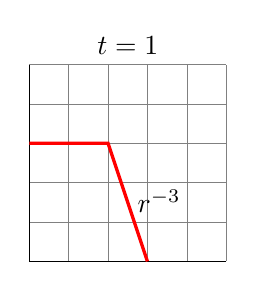
\begin{tikzpicture}
%					Tracé de la grille :
					\draw[step=.5cm,gray,very thin] (0,0) grid (2.5,2.5);
%					Tracé des axes :
					\draw (0,0) -- (0,2.5);
					\draw (0,0) -- (2.5,0);
%					Tracé du graphe :
					\draw[red,very thick] (0,1.5) -- (1,1.5) -- (1.5,0);
%					\draw[red,very thick] (1,1.5) -- (1.5,0);
					\draw (1.25,0.5) node[above right]{$r^{-3}$};
					\draw (1.25,2.5) node[above]{$t = 1$};
				\end{tikzpicture}
			\end{center}
		\end{minipage}\hfill
		\begin{minipage}[b]{0.24\linewidth}
			\begin{center}
				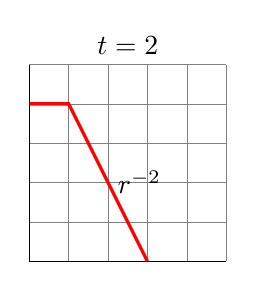
\begin{tikzpicture}
%					Tracé de la grille :
					\draw[step=.5cm,gray,very thin] (0,0) grid (2.5,2.5);
%					Tracé des axes :
					\draw (0,0) -- (0,2.5);
					\draw (0,0) -- (2.5,0);
%					Tracé du graphe :
					\draw[red,very thick] (0,2) -- (0.5,2) -- (1.5,0);
%					\draw[red,very thick] (0.5,2) -- (1.5,0);
					\draw (1,1) node[right]{$r^{-2}$};
					\draw (1.25,2.5) node[above]{$t = 2$};
				\end{tikzpicture}
			\end{center}
		\end{minipage}\hfill
		\begin{minipage}[b]{0.20\linewidth}
			\begin{center}
				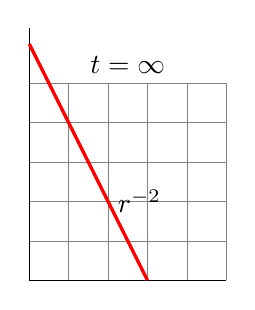
\begin{tikzpicture}
%					Tracé de la grille :
					\draw[step=.5cm,gray,very thin] (0,0) grid (2.5,2.5);
%					Tracé des axes :
					\draw (0,0) -- (0,3.2);
					\draw (0,0) -- (2.5,0);
%					Tracé du graphe :
					\draw[red,very thick] (0,3) -- (1.5,0);
					\draw (1,1) node[right]{$r^{-2}$};
					\draw (1.25,2.5) node[above]{$t = \infty$};
				\end{tikzpicture}
			\end{center}
		\end{minipage}
		\caption{Schéma d'évolution dynamique d'un amas globulaire.\label{schema-effondrement}}
	\end{figure}


%(~la pente $-4$ avec laquelle commence le schéma vient des résultats de simulations numériques~).
%La question à laquelle nous souhaitons répondre est : comment expliquer qu'un amas évolu en augmentant la densité de son cœur et en diminuant la pente avec laquelle le halo décroit ?

%Pour commencer, un amas doit, lorsqu'il est à l'équilibre, suivre un modèle de \textsc{King} ou de sphère isotherme en boîte. Par conséquent, notre amas est au Viriel.
%De plus, le cœur est un systéme auto-gravitant décrit par la thermodynamique. L'un de ses propriétés thermodynamique les plus importante à ce niveau est sa capacité calorifique. En effet :
%Nous cherchons à concentrer la matière dans le cœur de l'amas, et donc y rajouter de la matière à partir du halo (~qui va se diluer~).
%Pour faire diminuer le rayon de l'orbite d'un astre, il faut augmenter sa vitesse~\footnote{rappel : $v^2 = K\left(\frac{2}{r} - \frac{1}{a}\right)$ avec $K = G\left(M+m\right)$
%pour des interactions à deux corps}, et donc sa température. En se rappelant les résultats sur les diagrammes d'énergie de la sphère isotherme, nous nous rendons bien compte que, si la température
%augmente trop, le cœur va passer dans la zone instable, et s'effondrer.

%Le processus pour faire augmenter la température auquel nous nous attèlerons dans la suite est assez simple : l'amas évolue dans le potentiel galactique ; il va en traverser le disque de façon périodique.
%Moments pendant lesquels il va se faire harceler par des forces de marée qui vont lui faire perdre des étoiles. En considérant la description micro canonique, l'énergie est fixé ; or perdre une étoile
%diminue l'énergie potentielle de l'amas. La température va devoir augmenter pour conserver l'énergie totale constante.

%La perte d'étoile apparaît alors comme un processus intéressant pour expliquer l'évolution observée. Les chapitres suivants nous permettront de déterminer, à l'aide de simulation numérique, si la perte
%d'étoile par effet de marée est suffisante pour l'expliquer.








Cette dernière étude nous montre que plus un amas est âgé, plus la pente de son halo est importante.
Dans le chapitre précédent, nous avons relié la pente au paramètre $W_0$ qui, en plus de jouer sur les pentes, joue sur la densité centrale, comme le montre la figure~\ref{King_Modele-test}.
Par ailleurs, des simulations partant d'un nuage homogène nous apprennent que la pente du halo après sa formation vaut $-4$.
Un amas va donc partir d'une structure cœur-halo avec un cœur de taille importante, un halo de pente $-4$ et va tendre, en vieillissant, vers un amas ayant une densité centrale très élevée dont la pente tend vers $-2$.
Puis après un temps infini, l'amas va tendre vers une sphère isotherme.
C'est ce que représente le schéma suivant.


	\begin{figure}[ht!]
		\begin{minipage}[b]{0.20\linewidth}
			\begin{center}
				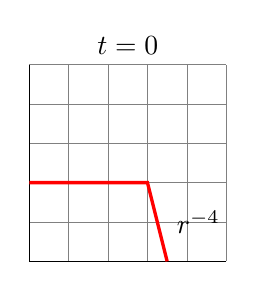
\begin{tikzpicture}
%					Tracé de la grille :
					\draw[step=.5cm,gray,very thin] (0,0) grid (2.5,2.5);
%					Tracé des axes :
					\draw (0,0) -- (0,2.5);
					\draw (0,0) -- (2.5,0);
%					Tracé du graphe :
					\draw[red,very thick] (0,1.0) -- (1.5,1.0) -- (1.75,0);
%					\draw[red,very thick] (1.5,1.0) -- (1.75,0);
					\draw (1.75,0.5) node[right]{$r^{-4}$};
					\draw (1.25,2.5) node[above]{$t = 0$};
				\end{tikzpicture}
			\end{center}
		\end{minipage}\hfill
		\begin{minipage}[b]{0.20\linewidth}
			\begin{center}
				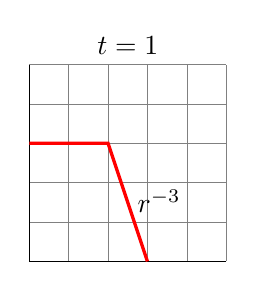
\begin{tikzpicture}
%					Tracé de la grille :
					\draw[step=.5cm,gray,very thin] (0,0) grid (2.5,2.5);
%					Tracé des axes :
					\draw (0,0) -- (0,2.5);
					\draw (0,0) -- (2.5,0);
%					Tracé du graphe :
					\draw[red,very thick] (0,1.5) -- (1,1.5) -- (1.5,0);
%					\draw[red,very thick] (1,1.5) -- (1.5,0);
					\draw (1.25,0.5) node[above right]{$r^{-3}$};
					\draw (1.25,2.5) node[above]{$t = 1$};
				\end{tikzpicture}
			\end{center}
		\end{minipage}\hfill
		\begin{minipage}[b]{0.24\linewidth}
			\begin{center}
				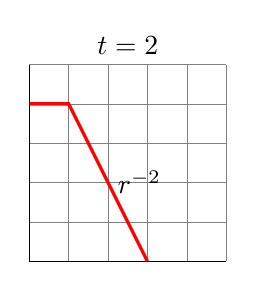
\begin{tikzpicture}
%					Tracé de la grille :
					\draw[step=.5cm,gray,very thin] (0,0) grid (2.5,2.5);
%					Tracé des axes :
					\draw (0,0) -- (0,2.5);
					\draw (0,0) -- (2.5,0);
%					Tracé du graphe :
					\draw[red,very thick] (0,2) -- (0.5,2) -- (1.5,0);
%					\draw[red,very thick] (0.5,2) -- (1.5,0);
					\draw (1,1) node[right]{$r^{-2}$};
					\draw (1.25,2.5) node[above]{$t = 2$};
				\end{tikzpicture}
			\end{center}
		\end{minipage}\hfill
		\begin{minipage}[b]{0.20\linewidth}
			\begin{center}
				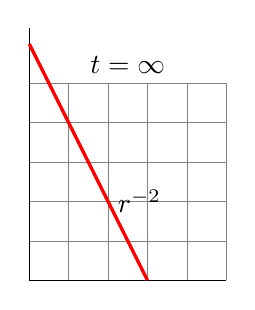
\begin{tikzpicture}
%					Tracé de la grille :
					\draw[step=.5cm,gray,very thin] (0,0) grid (2.5,2.5);
%					Tracé des axes :
					\draw (0,0) -- (0,3.2);
					\draw (0,0) -- (2.5,0);
%					Tracé du graphe :
					\draw[red,very thick] (0,3) -- (1.5,0);
					\draw (1,1) node[right]{$r^{-2}$};
					\draw (1.25,2.5) node[above]{$t = \infty$};
				\end{tikzpicture}
			\end{center}
		\end{minipage}
		\caption{Schéma d'évolution dynamique d'un amas globulaire.\label{schema-effondrement}}
	\end{figure}



Pour expliquer cette évolution, nous devons trouver quels phénomènes, de dynamique gravitationnelle, pourraient diluer le halo et concentrer de la matière au centre de l'amas. Le phénomène qui vient le plus naturellement à l'esprit est la perte d'étoiles, pouvant s'effectuer par 2 scénarios :
\begin{enumerate}
	\item des collisions internes qui éjectent des étoiles de l'amas, permettant ainsi au cœur de s'effondrer en essayant de compenser cette perte d'énergie.
	\item des interactions avec un autre objet massif qui va retirer par effet de marée des étoiles à l'amas, causant l'effondrement de son cœur.
\end{enumerate}
C'est ce deuxième scénario que nous allons tenter d'étudier.
















%Si la température cinétique du halo augmente, celle du
%cœur va changer pour s'adapter. La capacité calorifique à volume
%constant est négative pour le cœur (~et pour tout système
%auto gravitant~) :
%\begin{align*}
%	E_p &= -2E_c & \text{(~Viriel~)} \\
%	\Rightarrow E &= E_p + E_c = -E_c \\
%	\intertext{or}
%	E_c &\varpropto T \Rightarrow E\varpropto -T \\
%	\intertext{donc}
%	\Rightarrow C_v &= \frac{\partial E}{\partial T} < 0
%\end{align*}
%Cela implique que notre système ne peut que prendre de l'énergie.

%Si la température du cœur augmente, la vitesse de rotation des
%étoiles va augmenter (~$E_c\varpropto T\varpropto v$~), et donc
%leur demi grand axe va diminuer~\footnote{rappel : $v^2 =
%K\left(\frac{2}{r} - \frac{1}{a}\right)$ avec $K = G\left(M+m\right)$
%pour des interactions à deux corps}.
%En conséquent la densité au centre du cœur augmente, augmentant
%ainsi le contraste de densité. Si la température augmente
%suffisamment, le contraste de densité du halo va dépasser la
%valeur critique $\R_c^H$ (~l'énergie est fixé, seul la
%température change, nous utilisons donc la description micro
%canonique~). Le cœur va alors devenir instable.


%	L'interprétation semble simple ici : par exemple : quand les étoiles
%	ont des vitesses de rotation élevées la sphère a une température élevée,
%	et donc sa capacité calorifique à volume constant, $C_v = \frac{\partial H}{\partial T} < 0$
%	(~négatif car $E_p=-2E_c\Rightarrow H=E_c+E_p=-E_c\varpropto-T$~),
%	tend vers $0$ : elle ne peut plus acquérir d'énergie.
%	Si on dépasse la limite de température, elle va devoir se \og~réorganiser~\fg pour
%	rester à l'équilibre et donc pour retourner à un contraste de densité $\R < \R^\beta_c$.
%	Le raisonnement est le même pour la limite en énergie.


\chapter{Toy Model : Un modèle simplifié}
	\minitoc

	\section{Hypothèse et simplification}
			Nous avons dans le chapitre~\ref{King::Chapitre}, section~\ref{sec::temp}, le modèle de \King était un modèle
	quasi-isotherme ; il est de plus sphérique. Nous pouvons alors considérer ce modèle comme une sphère isotherme, en première
	approximation du moins. Par conséquent, il est possible de lui appliquer le problème d'Antonov. La première chose à
	faire est un rappel de ce qu'est l'instabilité d'Antonov.

\subsection{Problème/Instabilité d'Antonov}
	Le problème d'Antonov se pose lorsque l'on étudie la stabilité d'une sphère isotherme en boîte (voir
chapitre~\ref{SIB::Chapitre}) plongée dans un bain thermique.
%Ceci décale les tangentes de la spirale de stabilité.


	Cette explication de l'instabilité d'Antonov est grandement basée sur celle donnée
	dans~\cite{2008gady.book.....B}.

	Le problème que Antonov a posé est simple: supposons que le bord de la sphère isotherme en boîte soit un mur
conducteur et plaçons autour un bain thermique avec une température égale à celle de la sphère, pour commencer.
Si nous diminuons la température, nous déplaçons la sphère sur son diagramme Énergie--Température.
Par conséquent, nous changeons aussi le contraste de densité, qui est le paramètre de contrôle de la stabilité du
système.
Quand la température devient trop \og faible\fg, le contraste de densité devient trop important, et la sphère devient
instable.

	CHERCHER DES ARTICLES QUI PARLENT DE CATASTROPHE GRAVOTHERMALE (LYNDELL, BELL \& WOOD) ET D'INSTABILITE
	D'ANTONOV.

\subsection{Hypothèses simplificatrices}
	Nous avons étudié dans le chapitre~\ref{SIB::Chapitre} un modèle de sphère isotherme tronquée qui nous
	permettait une analyse de la stabilité de l'objet. Le problème est que ce modèle n'a rien d'analytique.
	Nous avons, à la fin de ce même chapitre, vu que l'objet avait un profil de densité $\rho(r)$ évoluant comme un
	cœur--halo, avec un halo ayant une pente $\alpha = 2$. L'idée de ce \og Toy-Model\fg est d'approximer le profil
	de densité comme :
	\begin{align}
		\rho(r) = \begin{cases}
			\rho_0	&	\text{si $<r_0$}\\
			\rho_0 \(\dfrac{R}{rx}\)^2	&	\text{si $r_0 < r \leq R$}\\
			0	&	\text{si $R < r$}
		\end{cases}
	\end{align}
	où $x = \frac{R}{r_0}$ est le contraste de densité, $\rho$ est la densité centrale de l'objet, $r_0$ le rayon de cœur, et $R$ le rayon de
	l'objet.

	Cette approximation permet de rendre compte des 2 tangentes discutées dans le chapitre~\ref{SIB::Chapitre}.

	Nous souhaitons appliquer ce problème à des fonctions de distributions pouvant être considérer comme des sphères
	isothermes (par exemple: la sphère de \King, en première approximation, section~\ref{sec::temp} et figure~\ref{King_Modele-test}).
	Nous allons donc approximer leur densité par:
	\begin{align}
		\rho(r) = \begin{cases} \rho_0 & \text{si $r < r_0$} \\
					\rho_0 \(\dfrac{R}{r}\)^\alpha \dfrac{1}{x^\alpha} & \text{si $R \geq r > r_0$, et
					$x=\frac{R}{r_0}$} \\
					0	&	\text{si $r > R$}
			  \end{cases}
	\end{align}
	où $\alpha$ est un entier donnant la pente du halo. Cette expression analytique nous permet de mener à bien la
	plupart des calculs, selon la valeur de $\alpha$.

	Les différentes valeurs de $\alpha$ vont permettre d'imiter la forme du profile de \King, et peuvent donc être
	rapprochées du paramètre $W_0$, de la même façon que dans~\ref{ssec::LinkBetween}.


	\section{Cas Général}
		Il est utile de préciser avant de commencer que tous ces calculs généraux sont valides pour $\alpha\geq 4$.
Les valeurs $\alpha = 3,\, 4$ faisant intervenir des logarithmes, il est nécessaire des les étudier à part.
\subsection{Normalisation}
	À partir de ces hypothèses, nous pouvons commencer par calculer $\rho_0$ en utilisant:
	\begin{align*}
		\int_0^R \rho(r) = M
	\end{align*}
	Un calcul rapide nous permet d'obtenir:
	\begin{align}
		\rho_0 = \frac{3 M x^{3+\alpha } (-3+\alpha )}{4 \pi  R^3 \left(-3 x^3+x^{\alpha } \alpha
\right)}
	\end{align}

\subsection{L'énergie potentielle}
	Elle se calcul bien, en utilisant:
	\begin{align}
		E_p &= -4\pi G \int_0^R r\rho(r)\mu(r) \dr \notag
		\intertext{Avec:}
		\mu(r) &= 4\pi\int_0^r r^2\rho(r)\dr \notag
	\end{align}
	Un calcul rapide nous donne alors:
	\begin{align}
%			E_p(x) = \begin{cases}
%					\dfrac{ r_0^2 M^2 }{60\pi \( \dfrac{1}{\alpha-3}\( 1-x^{3-\alpha} \) + \dfrac{1}{3} \)^2} & \text{si $r < r_0$} \\
%					\\
%					\dfrac	{M^2 \left( \frac		{\left(2 \alpha^2-8 \alpha+6 \right) x^{\alpha}}
%										{\left(2 \alpha^3-9 \alpha^2+10 \alpha\right) x^{\alpha}+\left(-6 \alpha^2+27 \alpha-30\right) x^3}
%								-    \frac	{\left(\left(2 \alpha^2-5 \alpha\right) x^{\alpha+2}+\left(6-3 \alpha\right) x^5\right)}
%										{\left(-6 \alpha^2+27 \alpha-30\right) x^{\alpha+3}+ \left(2 \alpha^3-9 \alpha^2+10 \alpha\right) x^{2 \alpha}}
%							      \right)}
%						{4 \pi r_0\left(\frac{1}{\alpha-3} \left(1 - x^{3-\alpha}\right)+\frac{1}{3}  \right)} & \text{si $r_0<r$}
%			\end{cases}
		E_p(x) &= \frac{3 G M^2 x (-3+\alpha ) \left(-15 x^5 (-2+\alpha )+5 x^{2+\alpha } \alpha  (-5+2 \alpha
)-x^{2 \alpha } (-3+\alpha ) \alpha  (1+2 \alpha )\right)}{5 R (-2+\alpha ) (-5+2 \alpha ) \left(-3
x^3+x^{\alpha } \alpha \right)^2}
	\end{align}


\subsection{Pression}
	Nous allons avoir besoin de la pression pour étudier le problème d'Antonov. Selon les conditions que nous souhaitons mettre sur le bord de la sphère, nous
	avons deux manière de calculer. Nous allons présenter les deux méthodes, mais les calculs ne
	seront donné que pour une méthode en particulier.
	%: celle qui s'applique à notre problème: un bain thermique, et donc un extérieur isotherme.

	\paragraph{Cas \og général\fg:} Dans le cas \og général\fg, nous appliquons
		l'équation de l'hydrostatique:
		\begin{align}
			\deriv{P}{r} = -\rho(r) \deriv{\psi}{r}
		\end{align}
		Le potentiel étant obtenu par résolution de l'équation de Poisson:
		\begin{align}
			\Delta\psi(r) = 4\pi G \rho(r)
		\end{align}
		En appliquant ces équations à notre problème simplifié, nous obtenons:
		\begin{align}
			P(R) &= \frac{3 G M^2 R^{-4-\alpha } x^3 (-3+\alpha ) \left(2 (R x)^{\alpha }
(-1+\alpha ) \alpha +R^{\alpha } x \left(-3 x^2 (1+\alpha )-x^{2 \alpha } (-3+\alpha ) \alpha  (2+\alpha
)\right)\right)}{8 \pi  \left(-3 x^3+x^{\alpha } \alpha \right)^2 \left(-1+\alpha ^2\right)}
		\end{align}
	\paragraph{Cas isotherme:} dans ce cas ci, l'équation de l'hydrostatique se
		ramène à l'équation d'un polytrope:
		\begin{align}
			P(r) &= \dfrac{\rho(r)}{m\beta}\\
			P(R) &= \frac{3 M \left(\frac{1}{x}\right)^{\alpha } x^{3+\alpha } (-3+\alpha )}{4 m \pi
R^3 \left(-3 x^3+x^{\alpha } \alpha \right) \beta }
		\end{align}

	\paragraph{Problème de définition:}
		Il nous faut maintenant définir de quelle pression nous parlons. En effet, dans un cas
		d'équilibre où les deux objets sont à la même température, le problème ne se pose pas: la
		continuité en pression impose qu'elle soit les mêmes au bord de la sphère. D'après la
		démonstration du théorème du Viriel pour une sphère (voir l'annexe~\ref{Demo::Viriel}, page~\pageref{Demo::Viriel}).

\subsection{Énergie cinétique}
	Ici encore, il y a deux méthodes de calculs, et ici encore, une seule
	sera décrite.
	\paragraph{Cas non-isotherme:} Dans ce cas, les calculs peuvent être très compliqué. En
		effet, ils nécessitent de connaître la fonction de distribution. Si elle n'est pas
		connue, il est possible de l'avoir en utilisant la formule d'Abel:
		\begin{align*}
			f(E) =
			\dfrac{1}{2\sqrt{2}\pi^2m^{7/2}}\(\int_0^E\deriv{\rho}{\phi}\dfrac{\mathrm{d\phi}}{\sqrt{E -
			m\phi}} + \dfrac{1}{\sqrt{E}} \left.\deriv{\rho}{\phi}\right\vert_{\phi=0}\)
		\end{align*}
		avec $\phi$ le potentiel et $\rho$ la densité.
		Ensuite, l'énergie cinétique se calcul alors simplement, pour peu que toutes les
		fonctions présentes soient analytique:
		\begin{align}
			E_c = \int_0^R\(\dfrac{1}{\rho(r)}\int \dfrac{p^2}{2m}f(E)\vdp\)\vdr
		\end{align}
	\paragraph{Cas isotherme:} Avec cette hypothèse, le calcul est \og on ne peut plus simple\fg:
		\begin{align}
			E_c = \dfrac{3M}{2m\beta}
		\end{align}

\subsection{Spirale de stabilité}
	Nous avons maintenant tous les ingrédients nécessaire, il va être nécessaire de les adimensionner. Nous allons utiliser
	les mêmes changements que pour la SIB:
	\begin{align}
		\mu     &= \dfrac{GMm\beta}{r_0x} \\
		\lambda &= \dfrac{HR}{GM^2}
	\end{align}
	où $H = E_c + E_p$ est l'énergie totale du système.

	Notre but étant d'obtenir ces deux quantités en fonction de $x$. L'énergie totale s'obtient facilement, en
	adimensionnant, mais nous auront besoin de la température. Pour la température, les calculs sont plus lourd: nous devons
	utiliser le théorème du Viriel adapté aux sphères. Ce qui nous donne l'équation suivante à résoudre:
	\begin{align}
		2E_c + E_p = \dfrac{4}{3}\pi R^3P_e
	\end{align}
	avec $P_e = P(R)$.

	Une fois ces deux quantités obtenues, il ne reste plus qu'à les tracer dans le plan $\(\lambda, \mu\)$.

	Ce qui nous amène à des courbes comme~\ref{ToyModel::AllAlpha}.
	\begin{figure}
		\centering \includegraphics[width=1\linewidth]{theorie/graphe/ToyModel-alpha_spirale.pdf}
		\caption{Diagramme Énergie-Température pour $\alpha=4, 5, 6, 7, 8$\label{ToyModel::AllAlpha}}
	\end{figure}

\subsection{Recherche des instabilité} % (fold)
	\label{sub:Recherche des instabilité}
	La recherche des instabilité se fait en recherchant les tangentes verticale et horizontal (si elles existent).
	Nous recherchons alors les points où :
	\begin{align}
		\deriv{\mu}{\lambda} &= 0
		\intertext{Soit :}
		\dfrac{\deriv{\mu(x)}{x}}{\deriv{\lambda(x)}{x}} &= 0
		\intertext{Donc :}
		\deriv{\mu(x)}{x} &= 0
	\end{align}
	Si il y a plusieurs solutions, il faut un moyen de les discriminer.
	En observant bien les courbes~\ref{ToyModel::AllAlpha}, nous nous rendons compte facilement que la tangente
	horizontale correspond toujours au maximum de la fonction $\mu(x)$. Nous devons donc chercher la valeur de $x$
	qui annule $\deriv{\mu(x)}{x}$ mais qui maximise $\mu(x)$.
% subsection Recherche des instabilité (end)


	\section{Cas $\alpha  = 4$}
		Plaçons nous dans le cas $\alpha=4$ :
\begin{align}
	\rho(r) &= \begin{cases}
			\rho_0	&	\text{si $r<r_0$}\\
			\rho_0 \(\dfrac{r_0}{rx}\)^4	&	\text{si $r > r_0$}
	\end{cases}
\end{align}
Nous utiliserons les résultats donnés dans la section précédente, en décrivant uniquement les cas où l'objet est
isotherme.
\subsection{Normalisation}
	En utilisant :
	\begin{align}
		\int_0^R \rho(r) &= M
	\end{align}
	La densité centrale $\rho_0$ va valoir :
	\begin{align}
		\rho_0 &= \dfrac{3}{4}\dfrac{M x^4}{R^3 \(4x - 3\) \pi}
	\end{align}
	Ainsi, la densité volumique de masse s'écrit :
	\begin{align}
			\rho(r) &= \begin{cases}
				\dfrac{3}{4}\dfrac{M x^4}{R^3 \(4x - 3\) \pi}  &       \text{si $r<r_0$}\\
				\dfrac{3}{4}\dfrac{M x^4}{R^3 \(4x - 3\) \pi}\(\dfrac{R}{rx}\)^4    &       \text{si $r >
				r_0$}
			\end{cases}
	\end{align}
	Il est alors possible d'en déduire la masse contenue dans un rayon $r$ :
	\begin{align}
		\mu\(r\) = \begin{cases}
			\dfrac{Mr^3x^4}{R^3\(4x-3\)}	&	\text{si $r < r_0$}\\
			\dfrac{\(3R-4rx\)M}{\(3-4x\)r}	&	\text{si $r>r_0$}
		\end{cases}
	\end{align}
\subsection{L'énergie potentielle}
	Sachant que:
	\begin{align}
		E_p(r) &= -4\pi G\int_0^r r\rho(r)\mu(r)\mathrm{dr}
		\intertext{Nous en déduisons l'énergie potentielle totale du système:}
		E_p^\mathrm{tot} &= -4\pi G\int_0^R r\rho(r)\mu(r)\mathrm{dr} \\
				 &= -\frac{3 G M^2 \left(5-10 x+6 x^3\right)}{5R (3-4 x)^2} \\
	\end{align}
\subsection{Énergie cinétique}
	Nous nous plaçons dans le cas où l'objet est isotherme (c'est le cas pour le modèle de \King, en première
	approximation). L'énergie cinétique s'écrit alors:
	\begin{align}
		E_c &= \dfrac{3M}{2m\beta}
	\end{align}
\subsection{Pression}
	Dans le cadre isotherme que nous utilisons, la pression s'exerçant sur la sphère est :
	\begin{align}
		P\(R\) = \frac{3 M}{4 m \pi  R^3 (-3+4 x) \beta }
	\end{align}
\subsection{Spirale de stabilité}
	En rappelant que le théorème du Viriel s'écrit :
	\begin{align}
		4\pi R^3 P(R) &= 2 E_c + E_p
	\intertext{pour une sphère isotherme, nous en déduisons la dépendance en $x$ de $\beta$ :}
		\beta(x) &= \frac{20R \left(3 -7  x+4  x^2\right)}{G m M \left(5-10 x+6 x^3\right)}
	\intertext{Nous en déduisons la dépendance de l'énergie avec $x$ :}
		E &= E_c + E_p^\mathrm{tot}
	\intertext{En utilisant les mêmes adimensionnements et notations que la SIS, nous arrivons à :}
		\mu(x) &= \frac{20 (-1+x) (-3+4 x)}{5-10 x+6 x^3}\\
		\lambda(x) &= -\frac{3 (-5+4 x) \left(5-10 x+6 x^3\right)}{40 (3-4 x)^2 (-1+x)}
	\end{align}

	Nous pouvons alors tracer le graphique~\ref{fig::DET}.

	\begin{figure}
		\centering \includegraphics[width=1\linewidth]{theorie/graphe/ToyModel-alpha4_spirale.pdf}
		\caption{Diagramme Énergie Température pour le Toy-Model, avec $\alpha=4$\label{fig::DET}}
	\end{figure}

\subsection{Recherche des instabilité}
	En appliquant la méthode décrite dans le cas général, nous trouvons que 4 valeurs de $x$ annule la dérivée
	première de $\mu(x)$ :
	\begin{align*}
		x =  \frac{1}{6} \left(3-\sqrt{3}\right), \frac{1}{6}
		\left(3+\sqrt{3}\right), \frac{1}{4} \left(5-\sqrt{5}\right),
		\frac{1}{4} \left(5+\sqrt{5}\right)
	\end{align*}

	La valeur de $x$ maximisant $\mu$ est : $x = \frac{1}{4} \left(5-\sqrt{5}\right)$.

\FloatBarrier


%	\section{Spirale de stabilité}
%		

%
%	\section{Recherche des instabilité}
%		


